\documentclass[mathserif,11pt]{beamer}
%%%%%%%%%%%%%%%%%%%%%%%%%%%%%%%%%%%%%%%%%%%%%%%%%%%%%%%%%%%%%%%%%%%%%%%%%%%%%%%%%%%%%%%%%%%%%%%%%%%%%%%%%%%%%%%%%%%
% Appearance
\mode<presentation>
{
	\usetheme{CambridgeUS}
	\usecolortheme{whale}
	\setbeamercovered{transparent}
}
% Redefine beamer colors
% Captions and titles
\setbeamertemplate{caption}{\raggedright\insertcaption} 
\setbeamercolor{frametitle}{fg=cyan!90!black}
\setbeamercolor{title}{bg=cyan!90!black}

\setbeamercolor{palette primary}{fg=white, bg=cyan!70!black}
\setbeamercolor{palette secondary}{fg=white, bg=cyan!50!black}
\setbeamercolor{palette tertiary}{fg=white, bg=cyan!90!black}
% Outline slide
\setbeamertemplate{section in toc}[circle]
\setbeamerfont{section number projected}{family=\rmfamily,series=\bfseries,size=\normalsize}
\setbeamercolor{section number projected}{bg=cyan!90!black,fg=white}
% Itemize list
\setbeamertemplate{itemize item}[circle]
\setbeamertemplate{itemize subitem}[circle]
\setbeamercolor{itemize item}{fg=cyan!70!black}
\setbeamercolor{itemize subitemitem}{fg=cyan!70!black}
% Title box
\setbeamertemplate{frametitle}{%
	\nointerlineskip%
	\begin{beamercolorbox}[wd=\paperwidth,ht=2.0ex,dp=0.6ex]{frametitle}
		\hspace*{1ex}\insertframetitle%
	\end{beamercolorbox}%
}
%%%%%%%%%%%%%%%%%%%%%%%%%%%%%%%%%%%%%%%%%%%%%%%%%%%%%%%%%%%%%%%%%%%%%%%%%%%%%%%%%%%%%%%%%%%%%%%%%%%%%%%%%%%%%%%%%%%
\usepackage[english]{babel}
% or whatever
\usepackage[latin1]{inputenc}
% or whatever
\usepackage{array} % To vertically center tabular content 
\usepackage{times}
\usepackage[T1]{fontenc}
%\usepackage{eulervm}
%\usepackage{cmbright}
%%%%%%%%%%%%%%%%%%%%%%%%%%%%%%%%%%%%%%%%%%%%%%%%%%%%%%%%%%%%%%%%%%%%%%%%%%%%%%%%%%%%%%%%%%%%%%%%%%%%%%%%%%%%%%%%%%%%
%\usepackage{tikz}
\usepackage{pgfplots}
\pgfplotsset{every axis/.append style={line width=1pt}}
\usetikzlibrary{shapes,shadows,arrows,backgrounds,patterns,positioning,automata,calc,decorations.markings,decorations.pathreplacing,bayesnet,arrows.meta}
\usepackage{amsmath,amssymb,mathrsfs,amsfonts,amsthm} % for maths
\usepackage{graphicx}
%\usepackage{subfig}
\usepackage{eucal}    % for curly math letter symbols
\usepackage{amssymb}  % for ams symbols
\usepackage{pifont}
\usepackage{color} %Invoke options usenames,dvipsnames for larger color choice
\usepackage{microtype} % Slightly tweak font spacing for aesthetics
\usepackage{multicol} % Used for the two-column layout of the document
\usepackage{smartdiagram}
\pgfplotsset{compat=1.12}
%%%%%%%%%%%%%%%%%%%%%%%%%%%%%%%%%%%%%%%%%%%%%%%%%%%%%%%%%%%%%%%%%%%%%%%%%%%%%%%%%%%%%%%%%%%%%%%%%%%%%%%%%%%%%%%%%%%%
\DeclareSymbolFontAlphabet{\mathcal} {symbols}
\DeclareSymbolFont{symbols}{OMS}{cm}{m}{n}
\DeclareMathAlphabet{\mathbfit}{OML}{cmm}{b}{it}
\newcommand\id{\ensuremath{\mathbbm{1}}} 
\DeclareMathOperator{\E}{\mathbb{E}}
\DeclareMathOperator{\eye}{\mathbb{I}}
\DeclareMathOperator{\zeros}{\mathbb{O}}
\DeclareMathOperator{\tr}{\textrm{tr}}
\DeclareMathOperator{\vvec}{\textrm{vec}}
\DeclareMathOperator{\ik}{\mathrm{k}}
\DeclareMathOperator{\ip}{\mathrm{p}}
\DeclareMathOperator{\inn}{\mathrm{n}}
\DeclareMathOperator{\im}{\mathrm{m}}
\DeclareMathOperator{\td}{\mathrm{t}}
\DeclareMathOperator{\kd}{\mathrm{k}}
\DeclareMathOperator{\T}{\mathrm{T}}
\DeclareMathOperator{\K}{\mathrm{K}}
%%%%%%%%%%%%%%%%%%%%%%%%%%%%%%%%%%%%%%%%%%%%%%%%%%%%%%%%%%%%%%%%%%%%%%%%%%%%%%%%%%%%%%%%%%%%%%%%%%%%%%%%%%%%%%%%%%%%
\usepackage[backend=bibtex,style=ieee]{biblatex} % bibliography
\bibliography{Bibliography-thesis}
\renewcommand*{\bibfont}{\footnotesize}
%%%%%%%%%%%%%%%%%%%%%%%%%%%%%%%%%%%%%%%%%%%%%%%%%%%%%%%%%%%%%%%%%%%%%%%%%%%%%%%%%%%%%%%%%%%%%%%%%%%%%%%%%%%%%%%%%%%%
\title[Identification of immune cell migration] % (optional, use only with long paper titles)
{Modelling and Identification of Immune Cell Migration during the Inflammatory Response}
\subtitle{PhD Viva}
\author[A. Kadochnikova]{A. Kadochnikova\inst{1}}
\institute[ACSE,TUoS]{\inst{1}
  Department of Automatic Control and Systems Engineering\\
  The University of Sheffield}
\date[01/07/2019]{1 July 2019}
%\date{\today}

\pgfdeclareimage[height=1cm]{university-logo}{UoSarms.pdf}
\logo{\pgfuseimage{university-logo}}

\begin{document}
\begin{frame}
  \titlepage
\end{frame}
%\begin{frame}{Outline}
%  \tableofcontents[hideallsubsections]
%  % You might wish to add the option [pausesections]
%\end{frame}

% - Exactly two or three sections (other than the summary).
% - At *most* three subsections per section.
% - Talk about 30s to 2min per frame. So there should be between about
%   15 and 30 frames, all told.


%% Chapters 1-2
\section[Background]{Background \& Objectives}
%\subsection{Neutrophils in inflammation}
%\begin{frame}
%\begin{figure}
%	\centering
%	\begin{tikzpicture}[->, >=stealth', auto, semithick, node distance=5em]
%	\tikzstyle{block} = [rectangle, draw, fill=white, 
%	text width=10em, text centered, rounded corners, minimum height=2em]
%	\tikzstyle{line} = [draw, -latex']
%	\draw[line width=0.5mm,cyan!90!black,fill=cyan!90!black,text centered, rounded corners] (0,7) rectangle (4.8,0);
%	\draw[line width=0.5mm,cyan!70!black,fill=cyan!70!black,text centered, rounded corners] (5.7,7) rectangle (10.5,0);
%	\node[align=center,text=white] at (2.4,6.5) (A2){Experimental studies};
%	\node[align=center,text=white] at (8.1,6.5) (A2){Mathematical models};
%	\draw[>=triangle 45,draw=cyan!50!black,line width=1pt, <->] (4.8,6.5) -- (5.7,6.5);	
%	\invisible<1-4>{\node[block,align=center] at (2.4,1) (A1){\small Sensing to motion\\ via subcellular signals};}
%	\invisible<1-3>{\node[block,align=center] at (2.4,2.5) (A2){\small Resolution via \\reverse migration};}
%	\invisible<1-2>{\node[block,align=center] at (2.4,4) (A3){\small \textit{in vivo} microscopy on zebrafish larvae};}
%	\invisible<1>{\node[block,align=center] at (2.4,5.5) (A4){\small Recruitment via chemotaxis};}
%	\invisible<1-8>{\node[block,align=center] at (8.1,1) (A5){\small Morphodynamics as intermediate level};}
%	\invisible<1-7>{\node[block,align=center] at (8.1,2.5) (A6){\small RDS models for subcellular species};}
%	\invisible<1-6>{\node[block,align=center] at (8.1,4) (A7){\small Random walk models for single cells};}
%	\invisible<1-5>{\node[block,align=center] at (8.1,5.5) (A8){\small RDS models for populations};}
%	\end{tikzpicture}
%\end{figure}
%\end{frame}
\subsection{Identified gaps in literature}
\begin{frame}{Neutrophils drive inflammatory response}
\begin{figure}
	\centering
	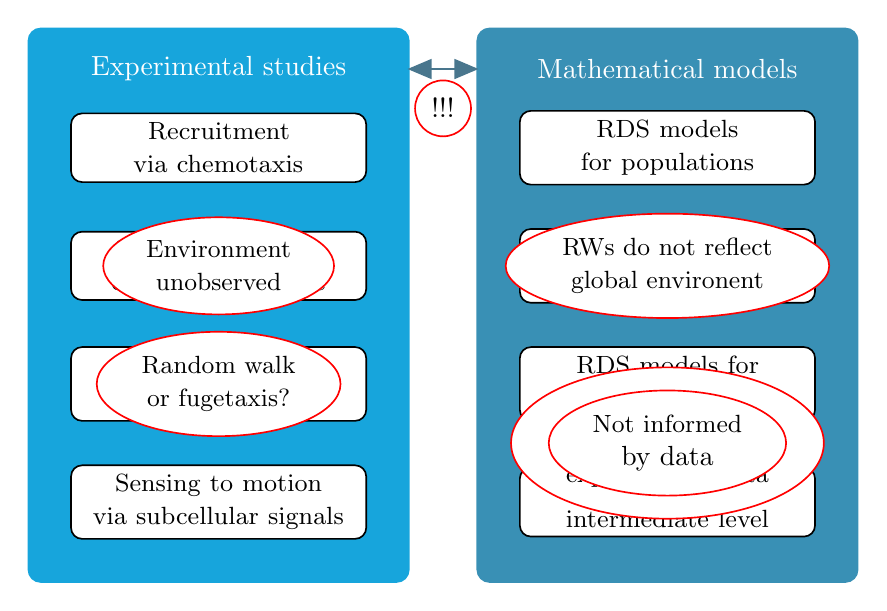
\begin{tikzpicture}[->, >=stealth', auto, semithick, node distance=5em]
	\tikzstyle{block} = [rectangle, draw, fill=white, 
	text width=10em, text centered, rounded corners, minimum height=2em]
	\tikzstyle{line} = [draw, -latex']
	\draw[line width=0.5mm,cyan!90!black,fill=cyan!90!black,text centered, rounded corners] (0,7) rectangle (4.8,0);
	\draw[line width=0.5mm,cyan!70!black,fill=cyan!70!black,text centered, rounded corners] (5.7,7) rectangle (10.5,0);
	\node[align=center,text=white] at (2.4,6.5) (A2){Experimental studies};
	\node[align=center,text=white] at (8.1,6.5) (A2){Mathematical models};
	\draw[>=triangle 45,draw=cyan!50!black,line width=1pt, <->] (4.8,6.5) -- (5.7,6.5);	
	\node[block,align=center] at (2.4,1) (A1){\small{Sensing to motion\\ via subcellular signals}};
	\node[block,align=center] at (2.4,2.5) (A2){\small{Resolution via \\reverse migration}};
	\node[block,align=center] at (2.4,4) (A3){\small \textit{in vivo} microscopy on zebrafish larvae};
	\node[block,align=center] at (2.4,5.5) (A4){\small Recruitment via chemotaxis};
	\node[block,align=center] at (8.1,1) (A5){\small Morphodynamics as intermediate level};
	\node[block,align=center] at (8.1,2.5) (A6){\small RDS models for subcellular species};
	\node[block,align=center] at (8.1,4) (A7){\small Random walk models for single cells};
	\node[block,align=center] at (8.1,5.5) (A8){\small RDS models for populations};
	\invisible<1>{\node[circle,draw=red,fill=white,align=center] at (5.25,6) (A0){!!!};}
	\invisible<1-2>{\node[ellipse,draw=red,fill=white,align=center] at (2.4,4) (A10){\small Environment \\ \small unobserved};}
	\invisible<1-3>{\node[ellipse,draw=red,fill=white,align=center] at (2.4,2.5) (A9){\small Random walk \\\small or fugetaxis?};}
	\invisible<1-4>{\node[ellipse,draw=red,fill=white,align=center] at (8.1,4) (A11){\small RWs do not reflect \\ \small global environent};}
	\invisible<1-5>{\node[ellipse,draw=red,fill=white,align=center] at (8.1,1.75) (A11){\small Models not\\ \small informed by \\ \small experimental data};}
	\invisible<1-6>{\node[ellipse,draw=red,fill=white,align=center] at (8.1,1.75) (A11){\small Not informed \\by data};}
	\end{tikzpicture}
\end{figure}
\end{frame}
\subsection{Research Objectives}
\begin{frame}
\begin{center}
\only<1>{\large{Common concept:\\ Complicated model $\rightarrow$ Realistic simulations.\\}}\only<2-3>{\large{Systematic approach:\\ Simplified models $\rightarrow$ Linking to data $\rightarrow$ Meaningful inferences.\\}}
\end{center}
\vspace{0.5cm}
\invisible<1-2>{Objectives:
	\begin{itemize}
		\item Develop a dynamical model that describes cell interaction with the global environment.
		\item Data-driven estimation of global chemoattractant concentration and cell behavioural modes.
		\item Parameter estimation of neutrophil morphodynamics model.
\end{itemize}}
\end{frame}
%% Chapters 3-5
\section{Environment inference: homogeneous cell behaviour}
\subsection{Problem statement}
\begin{frame}{Hidden chemoattractant}
\begin{columns}
	\begin{column}{0.55\textwidth}
		\centering
		\only<1-2>{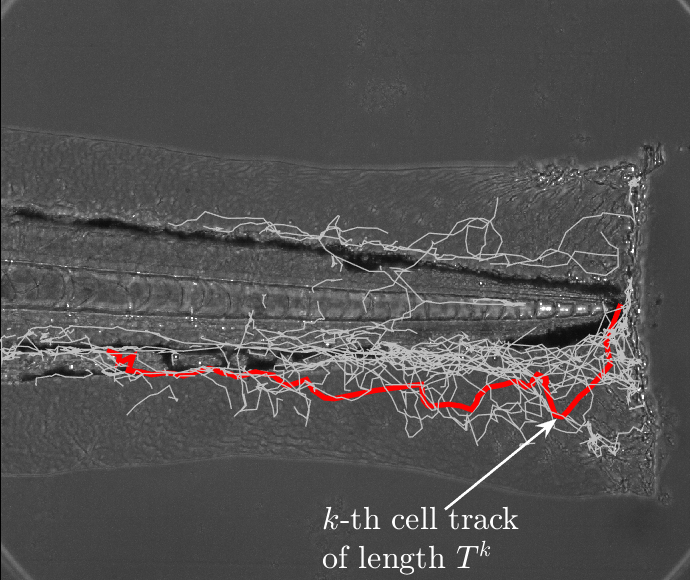
\includegraphics[scale=0.35]{Figures/track_k.png}}\only<3>{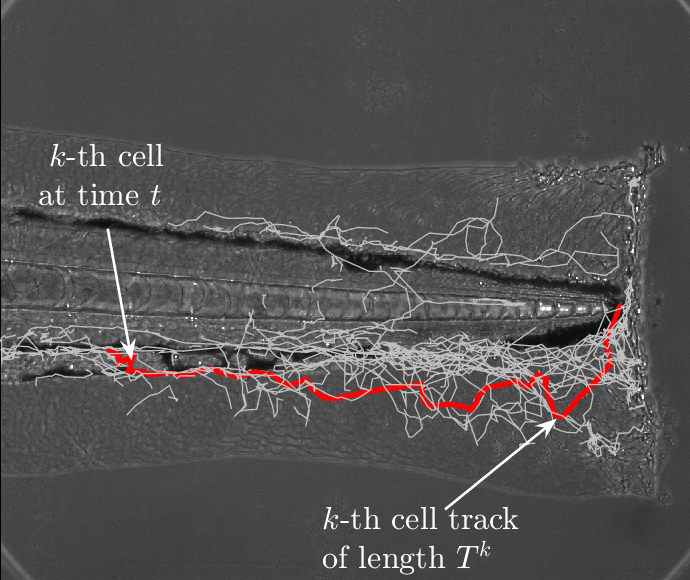
\includegraphics[scale=0.35]{Figures/track_k_time_t.png}}\only<4->{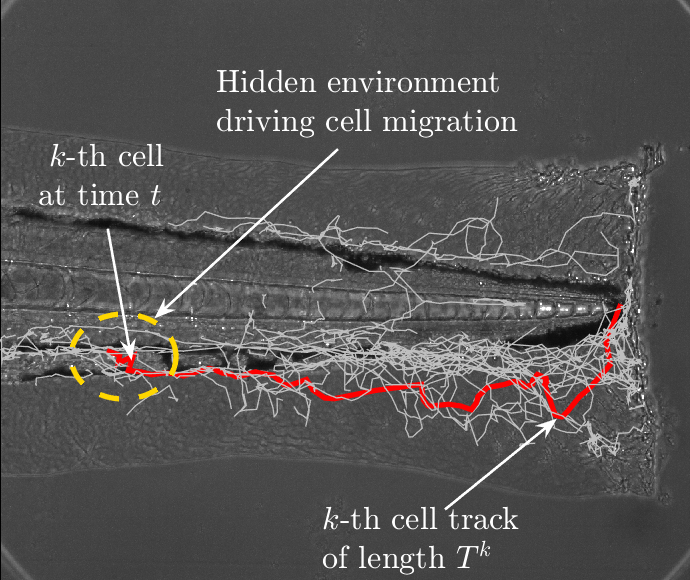
\includegraphics[scale=0.35]{Figures/track_filed.png}}
	\end{column}
	\begin{column}{0.42\textwidth}
		Time series data:
		\begin{itemize}
			\item<1-> $\K$ tracks: $\mathcal{Y} = \{\mathbf{y}^{\kd} \}^{\K}_{\kd=1}$
			\item<2-> Single track: $\mathbf{y}^{\kd} = \{ \mathbfit{y}^{\kd}_{\td}\}^{\T^{\kd}}_{\td=1}$
			\item<3-> Single data point: $\mathbfit{y}^{\kd}_{\td} = \left[ \bar{s}_{\mathrm{x}}, \bar{s}_{\mathrm{y}} \right]^{\top}$
%			\item<4-> Full state: $\mathbfit{x}^{k}_{t} = \left[ s_{\mathrm{x}}, s_{\mathrm{y}}, v_{\mathrm{x}}, v_{\mathrm{y}} \right]^{\top}$
			\item<4-> Environment influence:
			$\mathbfit{u}^{\kd}_{\td}  = \mathbfit{u}^{\kd}_{\td} (\mathbfit{s}) = \nabla \mathcal{U}(\mathbfit{s}).$
		\end{itemize}
	\end{column}
\end{columns}
\bigskip
\invisible<1-4>{1. Develop a parametrised finite-order model of global $\mathcal{U}(\mathbfit{s})$.\\}
\bigskip
\invisible<1-5>{2. Estimate unobserved $\mathcal{U}(\mathbfit{s})$ from localised tracking data $\mathcal{Y}$.}
\invisible<1-6>{\tiny{2. Estimate unobserved $\mathcal{U}(\mathbfit{s})$ from localised tracking data $\mathcal{Y}$.}}
\end{frame}
\begin{frame}{Defining assumptions}
\begin{itemize}
	\item<1-> A migrating call is moving as a massive Brownian particle:
	\begin{equation*}
	\dot{v}(t)= - \rho v(t) + \sqrt{\sigma}\mathbf{W}(t).
	\end{equation*}
	\item<2-> Each cell at each time is moving in response to the acting environment:
	\begin{equation*}
	\dot{v}(t) = - \rho v(t) + \sqrt{\sigma}\mathbf{W}(t) + {\psi}(t).
	\end{equation*}
	\item<3-> Hidden chemoattractant environment is acting on cells as a potential field:
	\begin{equation*}
	\dot{v}(t) = - \rho v(t) + \sqrt{\sigma}\mathbf{W}(t) + \mu\nabla\mathcal{U}(\mathbfit{s}(t)).
	\end{equation*}
	\item<4-> Hidden chemoattractant environment is time-invariant:
	\begin{equation*}
	\mathcal{U}(\mathbfit{s}(t)) = \mathcal{U}(\mathbfit{s}).
	\end{equation*}
\end{itemize}
\end{frame}
\subsection{Methods}
\begin{frame}{Decomposition of the environment}
\begin{columns}
\begin{column}{0.4\textwidth}
	\centering
	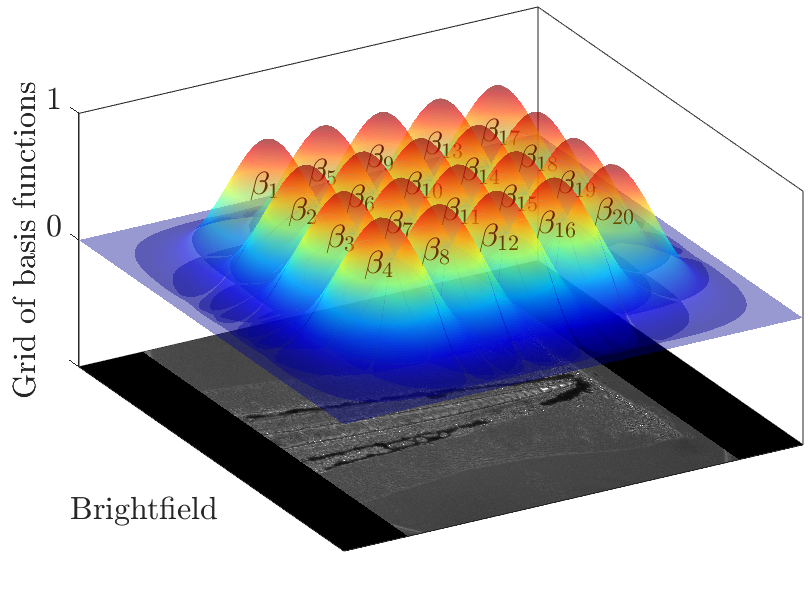
\includegraphics[scale=0.2]{Figures/grid.png}\\
	\footnotesize{a) 5x4 grid of tensor B-splines}
	\hfil
	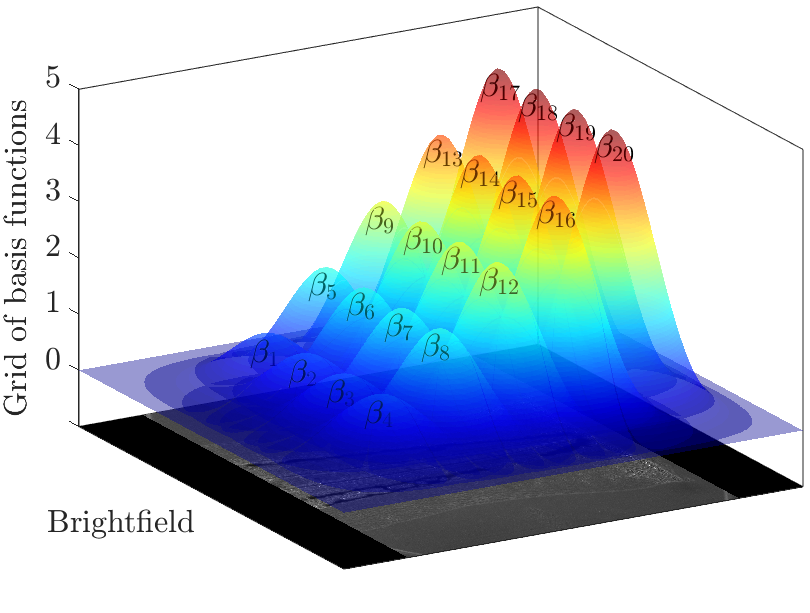
\includegraphics[scale=0.2]{Figures/grid2.png}\\
	\footnotesize{b) $\theta_h$ defines magnitude of $\beta_h (s_{\mathrm{x}}, s_{\mathrm{y}})$}
\end{column}
\begin{column}{0.5\textwidth}
	\centering
	\vspace{-0.5cm}
	\begin{equation*}\label{eq_field}
	\mathcal{U}(s_{\mathrm{x}}, s_{\mathrm{y}}) = \mathcal{B}\Theta = \sum_{h=1}^{N_b}\beta_h(s_{\mathrm{x}}, s_{\mathrm{y}})\theta_h,
	\end{equation*}
	\vspace{-0.5cm}
	\begin{subequations}
		\begin{eqnarray*}
		\Theta &= \left[\theta_1,\dots,\theta_h,\dots,\theta_{N_b}\right]^{\top},\\
		\mathcal{B} &= \left[\beta_1,\dots,\beta_h,\dots,\beta_{N_b}\right],\\
		\beta_h &(s_{\mathrm{x}}, s_{\mathrm{y}}) = \beta^{4}_{l}(s_{\mathrm{x}})\beta^{4}_{m}(s_{\mathrm{y}}).
		\end{eqnarray*}
	\end{subequations}

	\vfil
	\vspace{0.3cm}
	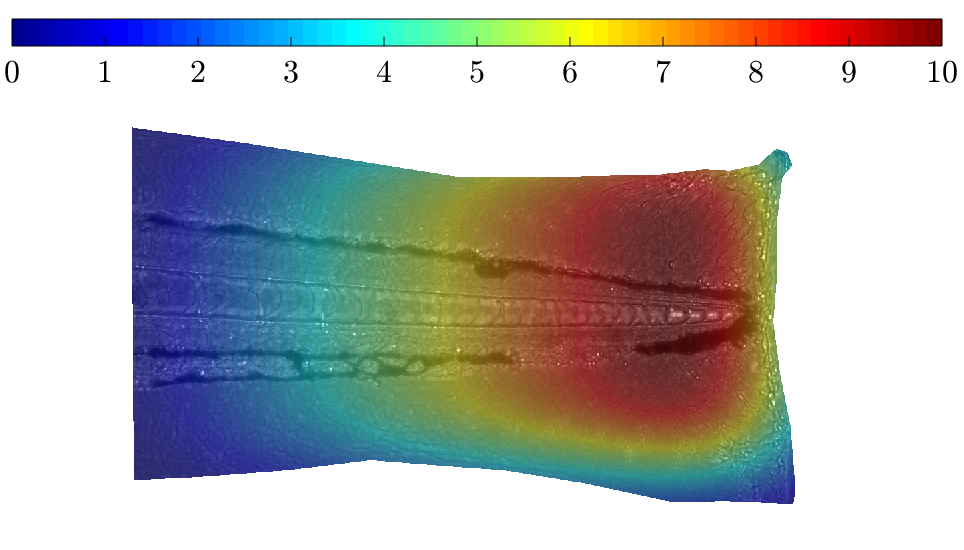
\includegraphics[scale=0.2]{Figures/grid_mask.png}\\
	\footnotesize{Example of the resultant field.}
\end{column}	
\end{columns}
\end{frame}
\begin{frame}{Model of neutrophil dynamics}
\vspace{-0.1cm}
Discrete time SSM of the $\kd$-th cell :
\begin{equation*}\label{eq_dyn}
\mathbfit{x}^{\kd}_{\td} = A \mathbfit{x}^{\kd}_{\td-1} + B\phi_{\td-1}^{\kd}(s_{\mathrm{x}},s_{\mathrm{y}}) \Theta + G\mathbfit{w}^{\kd}_{\td-1}, \quad \mathbfit{w}^{\kd}_{\td} \sim \mathcal{N}(0, Q)
\end{equation*}
\begin{equation*}\label{eq_meas}
\mathbfit{y}^{\kd}_{\td} = C\mathbfit{x}^{\kd}_{\td} + \mathbfit{v}^{\kd}_{\td}, \quad \mathbfit{v}^{\kd}_{\td} \sim \mathcal{N}(0, R)
\end{equation*}
where $\mathbfit{x}^{k}_{t} = \left[ s_{\mathrm{x}}, s_{\mathrm{y}}, v_{\mathrm{x}}, v_{\mathrm{y}} \right]^{\top}$,
\begin{equation*}
\phi_{\td}^{\kd}(s_{\mathrm{x}},s_{\mathrm{y}}) = \nabla \mathcal{B}(s_{\mathrm{x}}, s_{\mathrm{y}}) = \left[\begin{array}{ccccc} \frac{ \partial\beta_1(s_{\mathrm{x}},s_{\mathrm{y}}) }{\partial s_{\mathrm{x}}} &
 \dots &\frac{ \partial\beta_h(s_{\mathrm{x}},s_{\mathrm{y}}) }{\partial s_{\mathrm{x}}}& \dots&\frac{ \partial\beta_{N_b}(s_{\mathrm{x}},s_{\mathrm{y}}) }{\partial s_{\mathrm{x}}} \\
\frac{ \partial\beta_1(s_{\mathrm{x}},s_{\mathrm{y}}) }{\partial s_{\mathrm{y}}} & \dots &\frac{ \partial\beta_h(s_{\mathrm{x}},s_{\mathrm{y}}) }{\partial s_{\mathrm{y}}}& \dots&\frac{ \partial\beta_{N_b}(s_{\mathrm{x}},s_{\mathrm{y}}) }{\partial s_{\mathrm{y}}}
\end{array}\right]. 
\end{equation*}
\begin{equation*}
A = \left[\begin{array}{cc}
\eye & T\eye \\
\zeros & (1-T\rho) \eye
\end{array}\right]; 
\hfil 
B = \left[\begin{array}{c}
\zeros \\ T \eye
\end{array}\right];
\hfil
G = \left[ \begin{array}{c}
\zeros \\ T\eye
\end{array} \right]; 
\hfil
C = \left[ \begin{array}{cc}
\eye & \zeros
\end{array}\right].
\end{equation*}
%\vspace{0.3cm}
%SMM is linear with respect to $\Theta$ and non-linear with respect to $\mathbfit{x}$.   
\end{frame}
\begin{frame}{ML estimation with missing data}
%E-step:
%\vspace{-0.5cm}
%\begin{equation*}
%\mathcal{Q}(\Theta, \hat{\Theta}^i) = \E \big[\log p(\Theta \mid \mathcal{Y}) \big] = \E \Big[ \sum_{\kd=1}^{\K} \sum_{\td=1}^{\T_{\kd}}\log p(\mathbfit{x}_{\td}^{\kd} \mid \mathbfit{x}_{\td-1}^{\kd}, \Theta) \mid \mathcal{Y}, \hat{\Theta}^{i} \Big] + c.
%\end{equation*}
%\vspace{-0.2cm}
%\begin{equation*}
%p(\mathbfit{x}_{\td}^{\kd} \mid \mathbfit{x}_{\td-1}^{\kd} \Theta) = \mathcal{N}\big((G)^\dag \left\lbrace  \mathbfit{x}_{\td}^{\kd}- A\mathbfit{x}_{\td-1}^{\kd}- B\phi(C\mathbfit{x}_{\td-1}^{\kd}) \Theta\right\rbrace , \Sigma_{\mathbfit{w}}\footnote{\scriptsize{$\Sigma_{\mathbfit{w}} \triangleq \big\{(G)^\dag \big\}^\top (Q_{\omega})^{-1} (G)^\dag$}}\big).
%\end{equation*}
%\vfil
%Forecasting step:
%\vspace{-0.2cm}
%\begin{equation*}
%\mathbfit{s}_{\td}^{\kd} = C \hat{\mathbfit{x}}_{\td \mid \T^{\kd}}^{\kd}, \quad \td = 1, \dots, \T^{\kd}, \kd = 1, \dots, \K.
%\end{equation*} 
%\vspace{-0.4cm}
%\begin{equation*}
%\begin{split}
%p(\mathbfit{x}_{\td}^{\kd} \mid \mathbfit{x}_{\td-1}^{\kd}, \Theta) &\approx p(\mathbfit{x}_{\td}^{\kd} \mid \mathbfit{x}_{\td-1}^{\kd}, \mathbfit{s}_{\td-1}^{\kd}, \Theta)\\ &=   \mathcal{N}\big((G)^\dag\left\lbrace  \mathbfit{x}_{\td}^{\kd}- A\mathbfit{x}_{\td-1}^{\kd}- B\phi(\mathbfit{s}_{\td-1}^{\kd}) \Theta\right\rbrace, \Sigma_{\mathbfit{w}}\big).
%\end{split}
%\end{equation*}
%M-step:\\
%\vspace{-0.5cm}
%\begin{equation*}
%\hat{\Theta}^{i+1} = \arg \underset{\Theta}{\max} \tilde{\mathcal{Q}}(\Theta, \hat{\Theta}^i).
%\end{equation*}
%\end{frame}
%\begin{frame}
\begin{figure}
	\centering
	\begin{tikzpicture}[->, >=stealth', auto, semithick, node distance=5em]
	\tikzstyle{block} = [rectangle, draw, fill=white, 
	text width=7em, text centered, rounded corners, minimum height=2em]
	\tikzstyle{line} = [draw, -latex']	
	\node[block,align=center] at (1.5,6.2) (A1){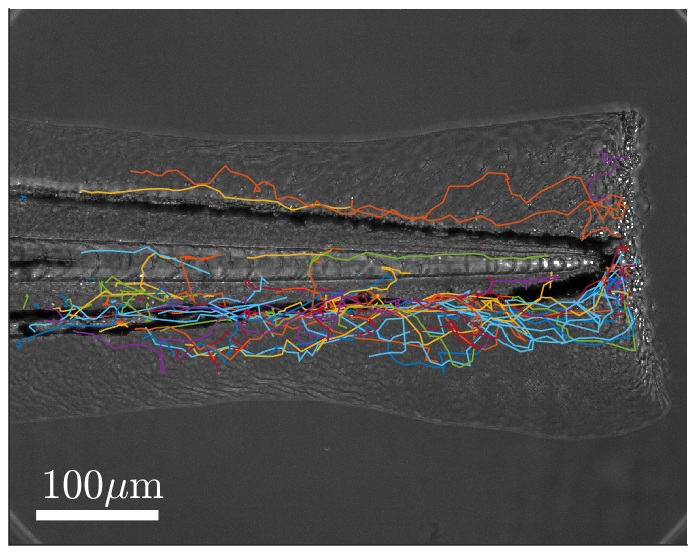
\includegraphics[width=.95\textwidth]{Figures/tracks_3.png}};
	\node[block,align=center] at (1.5,4.45) (A2){SSM};
	\node[block,align=center] at (1.5,2.8) (A3){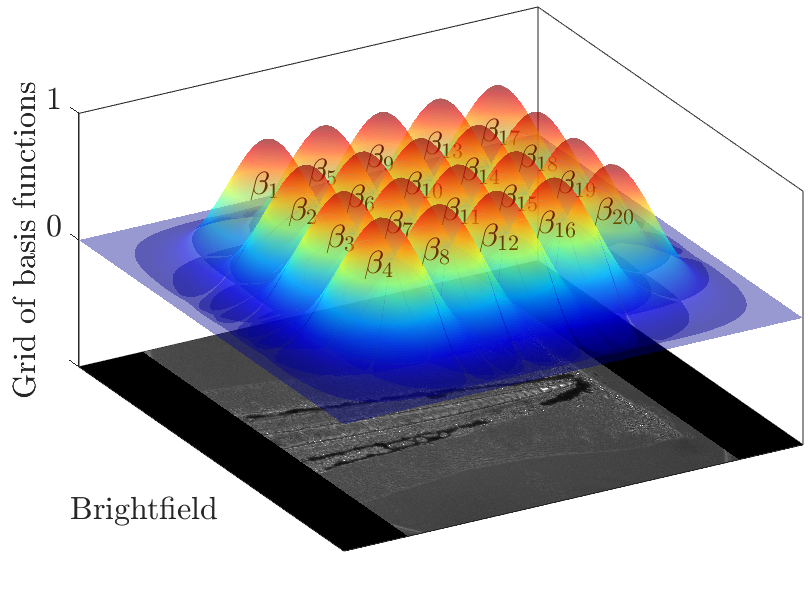
\includegraphics[width=.95\textwidth]{Figures/grid.png}};
	\node[align=center] at (5.75,6.8) (A4){\small Approximate \\ML framework};
	\node[block,align=center] at (5.6,5.8) (A5){\small  URTS: $\mathcal{X} \mid \hat{\Theta}^{i}$};
	\node[block,align=center] at (5.6,4.3) (A15){\small Forecasting $\mathcal{S} \mid \mathcal{X}, \hat{\Theta}^{i}$};
	\node[block,align=center] at (5.6,2.7) (A6){\footnotesize $\hat{\Theta}^{i+1} = \arg \underset{\Theta}{\max} \tilde{\mathcal{Q}}(\mathcal{X},\mathcal{S})$};
	\node[block,align=center] at (10,5.8) (A7){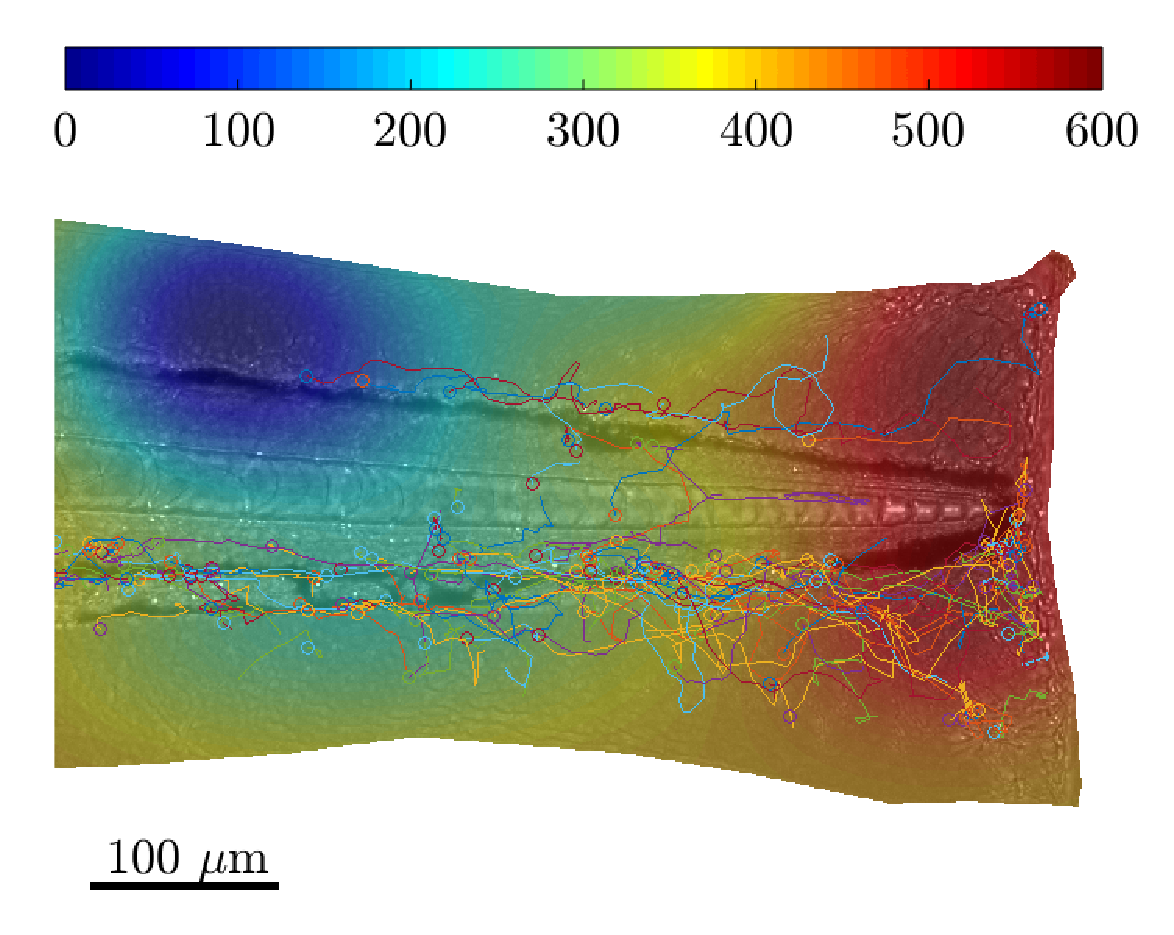
\includegraphics[width=.95\textwidth]{Figures/field_tracks_1.png}};
	\node[block,align=center] at (10,3.25) (A8){Cell velocities};
	\draw[line width=0.5mm,cyan!70!black, rounded corners] (3.55,7.3) rectangle (7.95,1.8);
	\node at (3.7,6.2) (A9){};
	\node at (3.7,2.8) (A10){};
	\node at (3.7,4.45) (A11){};
	\node at (7.8,5.8) (A12){};
	\node at (7.8,3.25) (A13){};
	%% arrows
	\draw (A1) -- (A9); 
	\draw (A2) -- (A11); 
	\draw (A3) -- (A10); 
	\draw (A12) -- (A7); 
	\draw (A13) -- (A8); 
	%	\path
	%	(A5.east) edge[dashed,bend left=30] (A6.east);
	\path
	(A5.south) edge[dashed] (A15.north);
	\path
	(A15.south) edge[dashed] (A6.north);
	\path
	(A6.east) edge[dashed,bend right=30] (A5.east);
	\end{tikzpicture}
\end{figure}
\end{frame}
\subsection{Selected results}
\begin{frame}{Inferred chemoattractant concentration}
\begin{columns}
	\begin{column}{0.3\textwidth}
		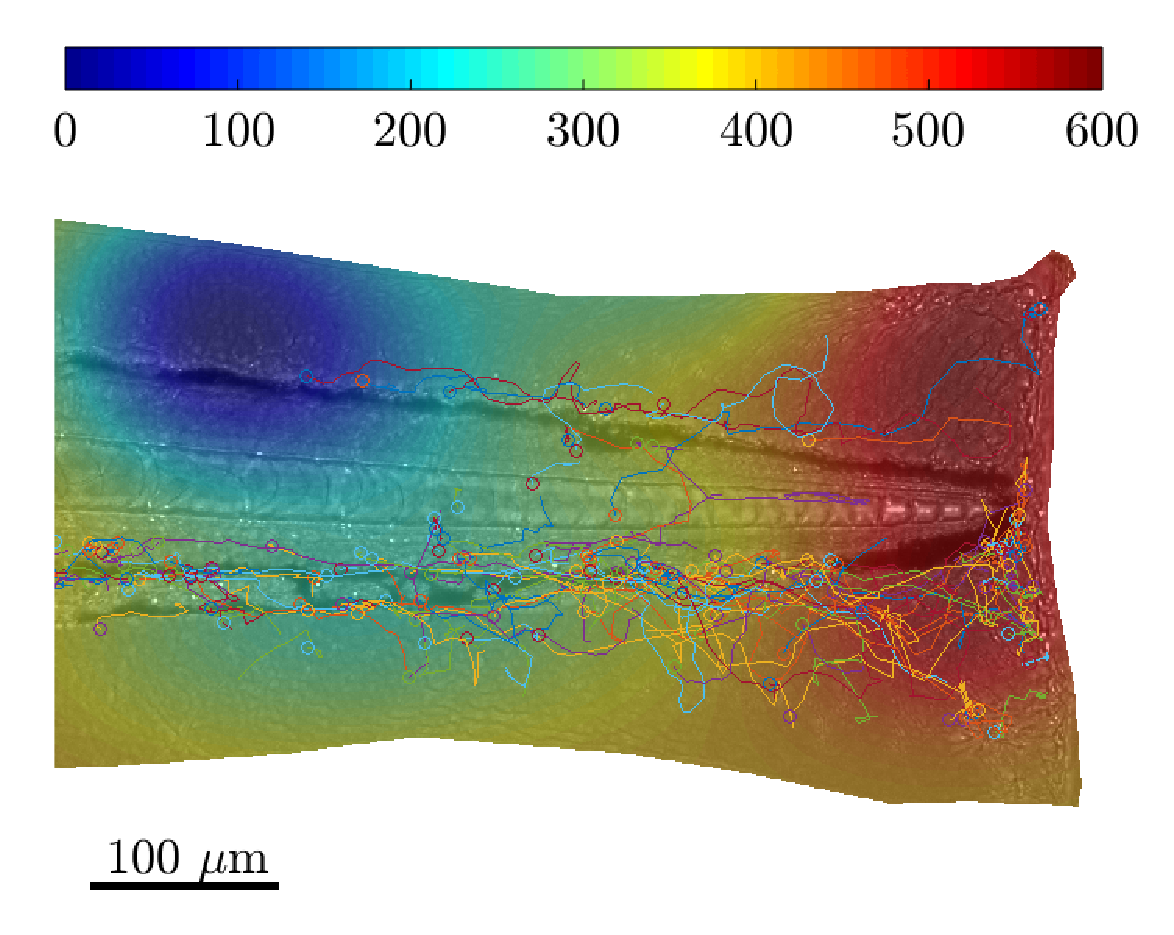
\includegraphics[scale=0.19]{Figures/field_tracks_1.png}
		\vspace{0.4cm}
		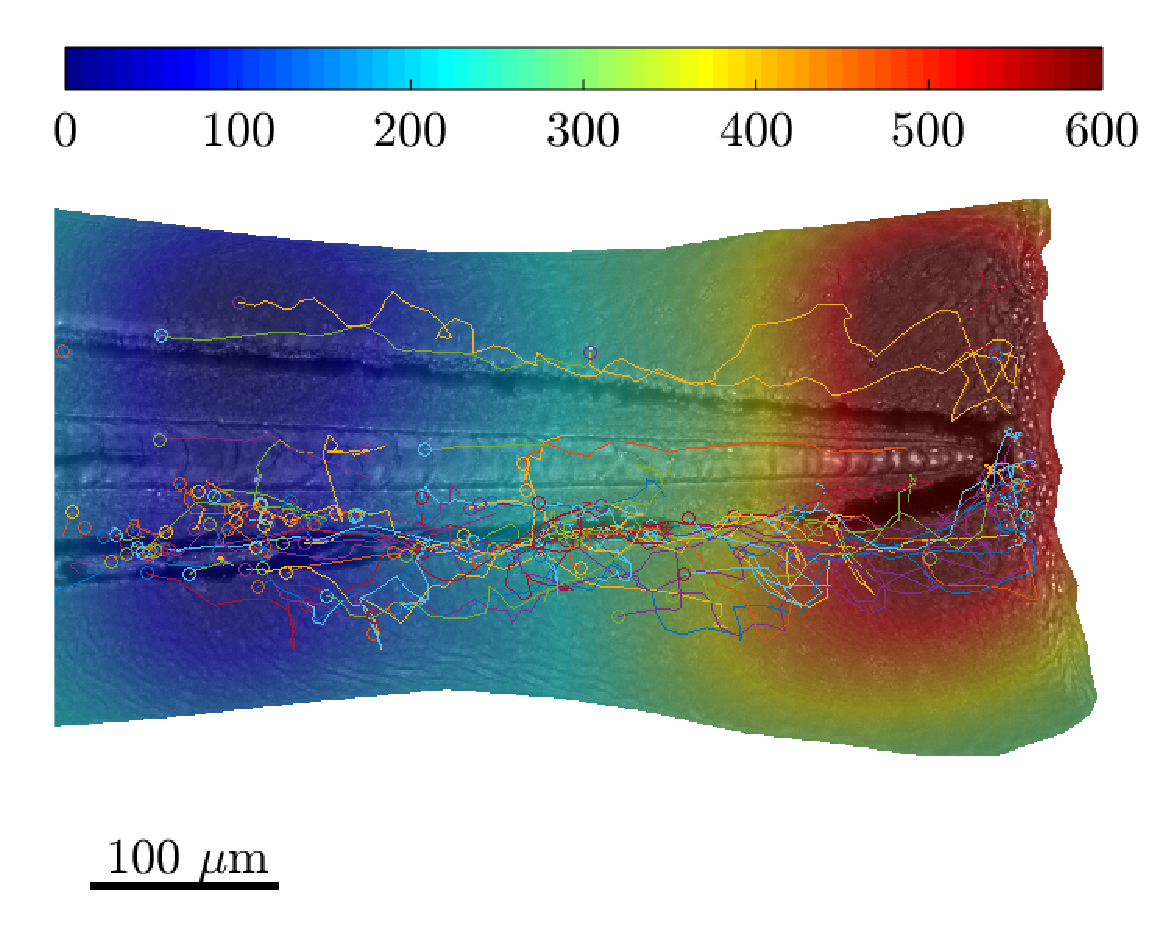
\includegraphics[scale=0.19]{Figures/field_tracks_3.png}
	\end{column}
	\begin{column}{0.3\textwidth}
		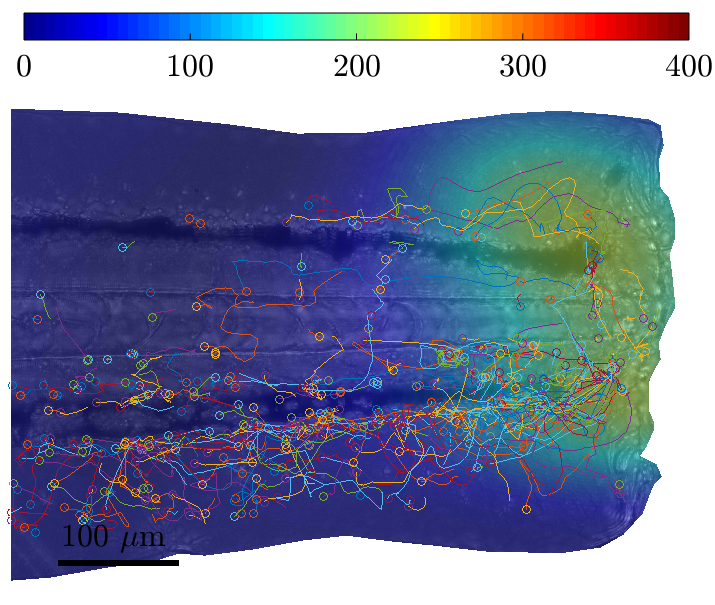
\includegraphics[scale=0.185]{Figures/s2_ukf_tracks.png}
		\vspace{0.3cm}
		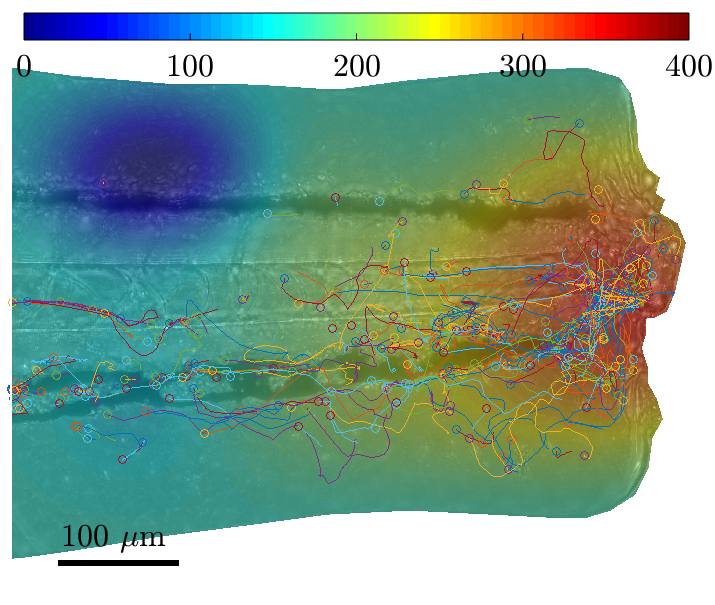
\includegraphics[scale=0.185]{Figures/s3_ukf_tracks.png}
	\end{column}
	\begin{column}{0.3\textwidth}
		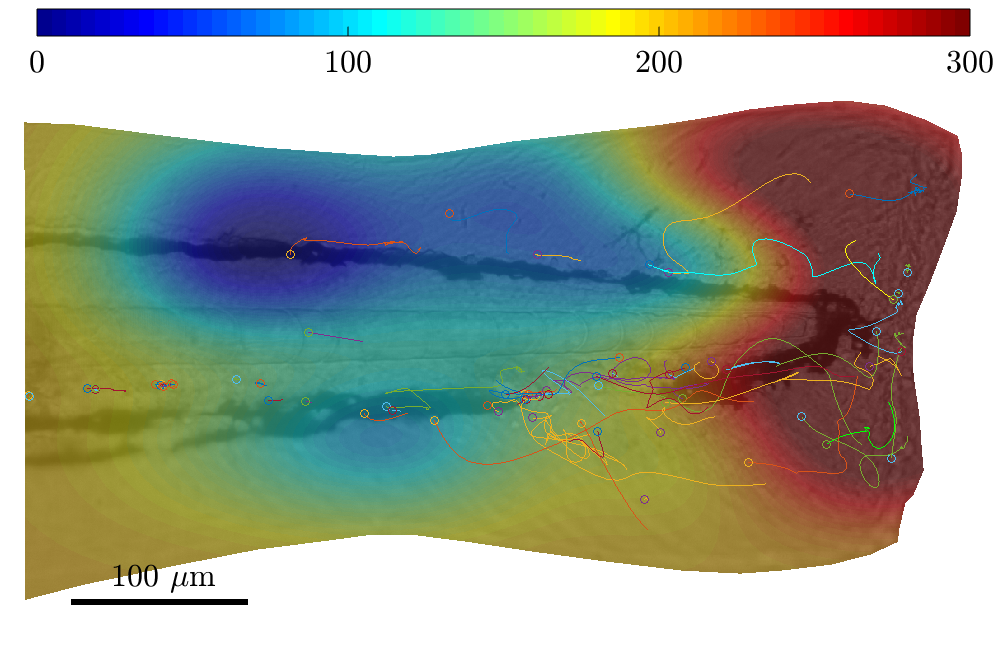
\includegraphics[scale=0.14]{Figures/n3_p1_ukf_tracks.png}
		\vspace{0.6cm}
		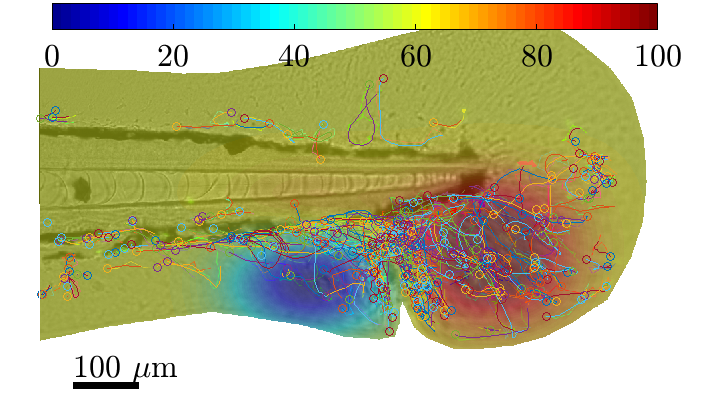
\includegraphics[scale=0.2]{Figures/nick4_4x4_05.png}
	\end{column}
\end{columns}
\begin{columns}
	\begin{column}{0.3\textwidth}
		\centering
		\footnotesize{ a) normal injury}\\
		\footnotesize{(6 datasets)}
	\end{column}
	\begin{column}{0.3\textwidth}
		\centering
	\footnotesize{ b) severe injury}\\
	\footnotesize{(2 datasets)}
\end{column}
	\begin{column}{0.3\textwidth}
		\centering
	\footnotesize{ c) mild injury}\\
	\footnotesize{(6 datasets)}
\end{column}
\end{columns}
\end{frame}
\begin{frame}{Estimated cell velocities}
\begin{columns}
	\begin{column}{0.32\textwidth}
		\scalebox{0.7}{\input{Tikzes/histogram_vx.tikz}}\vfil
		\scalebox{0.7}{\input{Tikzes/histogram_vy.tikz}}
	\end{column}
	\begin{column}{0.3\textwidth}
		\scalebox{0.7}{\input{Tikzes/histogram_vx_severe.tikz}}\vfil
		\scalebox{0.7}{\input{Tikzes/histogram_vy_severe.tikz}}
	\end{column}
	\begin{column}{0.3\textwidth}
		\scalebox{0.7}{\input{Tikzes/histogram_vx_nicked.tikz}}\vfil
		\scalebox{0.7}{\input{Tikzes/histogram_vy_nicked.tikz}}
	\end{column}
\end{columns}
\begin{columns}
	\centering
	\begin{column}{0.32\textwidth}
		\centering
		\footnotesize{ a) normal injury}
	\end{column}
	\begin{column}{0.3\textwidth}
		\centering
		\footnotesize{ b) severe injury}
	\end{column}
	\begin{column}{0.3\textwidth}
		\centering
		\footnotesize{ c) mild injury}
	\end{column}
\end{columns}
\end{frame}
%\begin{frame}{Cell modes}
%Neutrophil behaviour during recruitment stage can be described by a set of models.
%\begin{columns}
%	\begin{column}{0.5\textwidth}
%		Types of random walk \cite{Jones2015}:
%		\begin{itemize}
%			\item biased, persistent
%			\item biased, non-persistent
%			\item non-biased, persistent
%			\item non-biased, non-persistent
%		\end{itemize}
%	\end{column}
%	\begin{column}{0.5\textwidth}
%		Based on the interaction \\with the environment:
%		\begin{itemize}
%			\item driven by the field
%			\begin{itemize}
%				\item KS model
%				\item Potential Field model
%			\end{itemize}
%			\item insensitive - RW
%			\item stationary - RW
%		\end{itemize}
%		
%	\end{column}
%\end{columns}
%\end{frame}

\section{Environment inference: heterogeneous cell behaviour}
\subsection{Problem statement}
\begin{frame}{Heterogeneous cell behaviour}
\begin{columns}
	\begin{column}{0.5\textwidth}
		\centering
		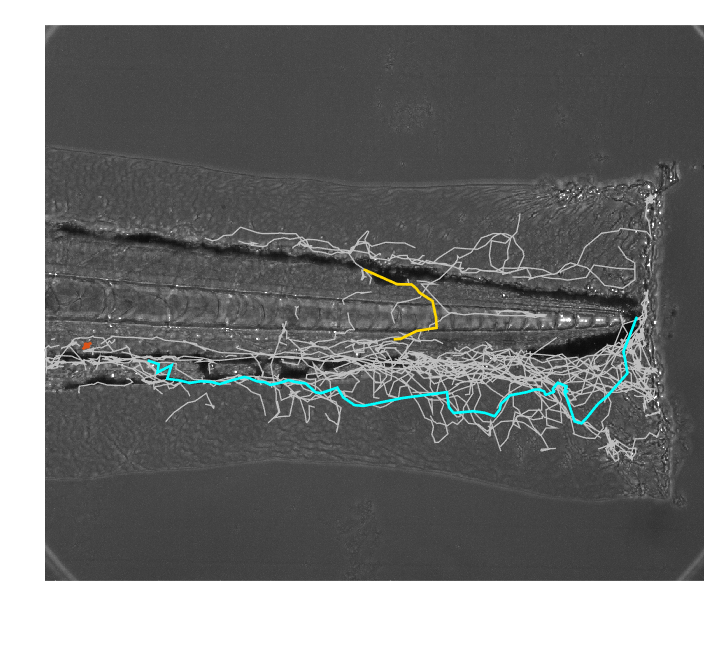
\includegraphics[scale=0.31]{Figures/example_tracks.png}
	\end{column}
	\begin{column}{0.5\textwidth}
		\centering
		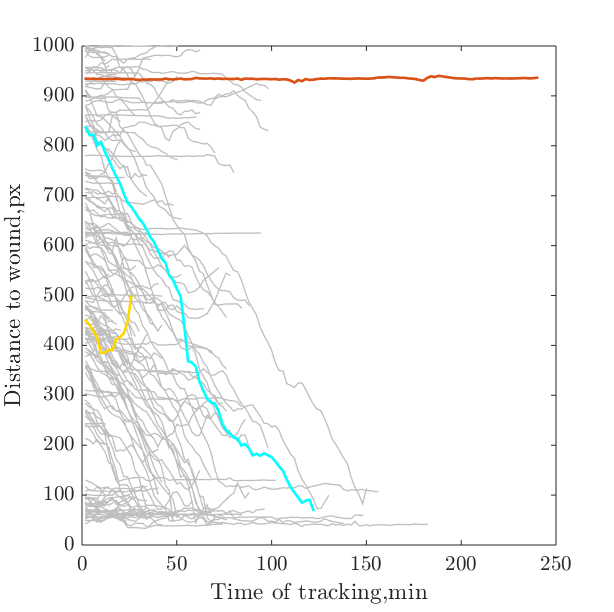
\includegraphics[scale=0.34]{Figures/example_distances.png}
		\vspace{0.29cm}
	\end{column}
\end{columns}
\invisible<1>{1. Determine whether a cell at a given time interacts with the environment $\mathcal{U}(\mathbfit{s})$.\\}
\vspace{0.2cm}
\invisible<1-2>{2. Estimate unobserved $\mathcal{U}(\mathbfit{s})$ from the interaction with responsive  cells.}
\invisible<1-3>{\tiny{2. Estimate unobserved $\mathcal{U}(\mathbfit{s})$ from the interaction with responsive  cells.}}

\end{frame}
\begin{frame}{Defining assumptions (upd.)}
Previous assumption:\\
Each cell at each time is moving in response to the acting environment.
\vfil
\vspace{0.5cm}
\uncover<2->{Relaxed assumptions:
\begin{itemize}
	\item Each migrating cell has modes: stationary, responsive or non-responsive.
	\item Switching between modes happens randomly.
	\item Each behavioural mode can be reached from any other mode.
\end{itemize}}
\end{frame}
\subsection{Methods}
\begin{frame}{Jump Markov system}
\vspace{-1cm}
\begin{equation*}
\begin{split}
\mathbfit{x}_{\td}^{\kd} &= A(\mathbfit{m}_{\td}^{\kd})\mathbfit{x}_{\td-1}^{\kd} + B(\mathbfit{m}_{\td}^{\kd})\phi_{\td-1}^{\kd}(s_{\mathrm{x}},s_{\mathrm{y}}) \Theta + G(\mathbfit{m}_{\td}^{\kd})\mathbfit{w}_{\td-1}^{\kd}, \\
\mathbfit{w}_{\td}^{\kd} &\sim \mathcal{N}(0,Q(\mathbfit{m}_{\td}^{\kd})), \\
\mathbfit{m}_{\td}^{\kd} &\in \left\lbrace M^1,M^2,M^3\right\rbrace .
\end{split}
\end{equation*}
\begin{columns}
	\begin{column}{0.45\textwidth}
		\centering
	\small{
	Cell modes:
	\begin{align*}
	M^1&: A = \left[\begin{array}{cc}
	\eye & T\eye \\
	\zeros & (1-T\rho(M^1)) \eye
	\end{array}\right] 
	\hfil 
	B = \left[\begin{array}{c}
	\zeros \\ T \eye
	\end{array}\right]
	\\
	M^2&: A = \left[\begin{array}{cc}
	\eye & T\eye \\
	\zeros & (1-T\rho(M^2)) \eye
	\end{array}\right]
	\hfil 
	B = \left[\begin{array}{c}
	\zeros \\ \zeros
	\end{array}\right]
	\\
	M^3&: A = \left[\begin{array}{cc}
	\eye & T\eye \\
	\zeros & (1-T\rho(M^3)) \eye
	\end{array}\right]
	\hfil 
	B = \left[\begin{array}{c}
	\zeros \\ \zeros
	\end{array}\right]
	\\
	Q&(M^3) \ll Q(M^1), Q(M^2).
	\end{align*}
}
\end{column}
\begin{column}{0.45\textwidth}
	\scalebox{0.58}{\input{Tikzes/Markov_chain_switch.tikz}}
\end{column}
\end{columns}
\end{frame}

\begin{frame}{Inference framework}
\begin{figure}
	\centering
	\begin{tikzpicture}[->, >=stealth', auto, semithick, node distance=5em]
	\tikzstyle{block} = [rectangle, draw, fill=white, 
	text width=7em, text centered, rounded corners, minimum height=2em]
	\tikzstyle{line} = [draw, -latex']	
	\node[block,align=center] at (1.5,6.2) (A1){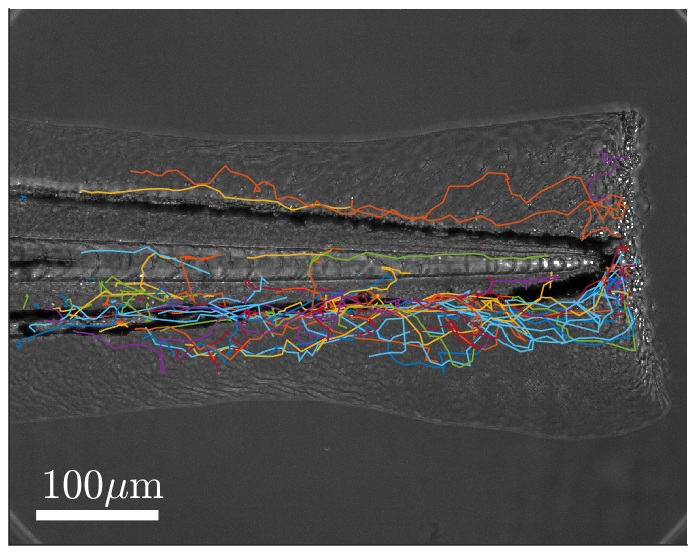
\includegraphics[width=.95\textwidth]{Figures/tracks_3.png}};
	\node[block,align=center] at (1.5,4.45) (A2){$\{M^1, M^2, M^3\}$};
	\node[block,align=center] at (1.5,2.8) (A3){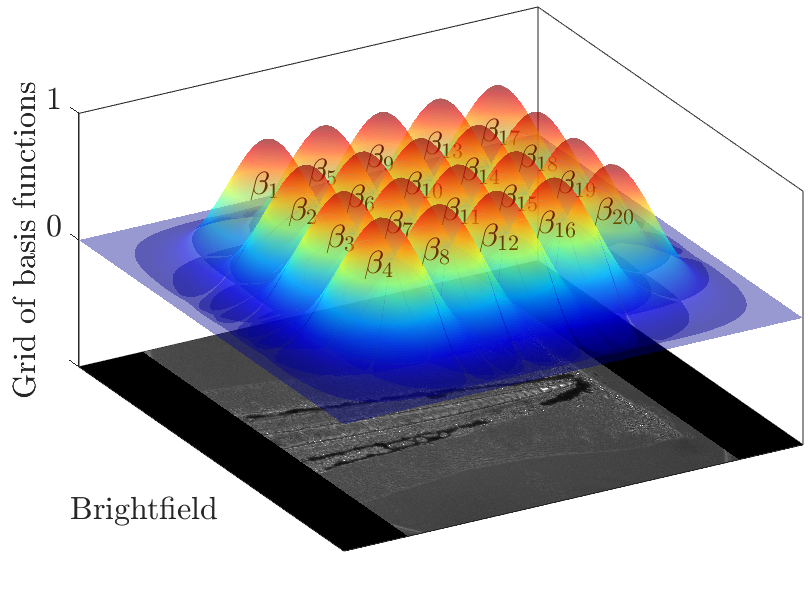
\includegraphics[width=.95\textwidth]{Figures/grid.png}};
	\node[align=center] at (5.75,6.9) (A4){\small Approximate ML framework};
	\node[block,align=center] at (5.6,5.9) (A5){\small  MM smoother $\mathcal{X},\mathcal{M} \mid \hat{\Theta}^{i}$};
	\node[block,align=center] at (5.6,4.4) (A15){\small Forecasting $\mathcal{S} \mid \mathcal{X}, \hat{\Theta}^{i}$};
	\node[block,align=center] at (5.6,2.8) (A6){\footnotesize $\hat{\Theta}^{i+1} = \arg \underset{\Theta}{\max} \tilde{\mathcal{Q}}(\mathcal{X},\mathcal{M},\mathcal{S})$};
	\node[block,align=center] at (10,5.8) (A7){\only<1>{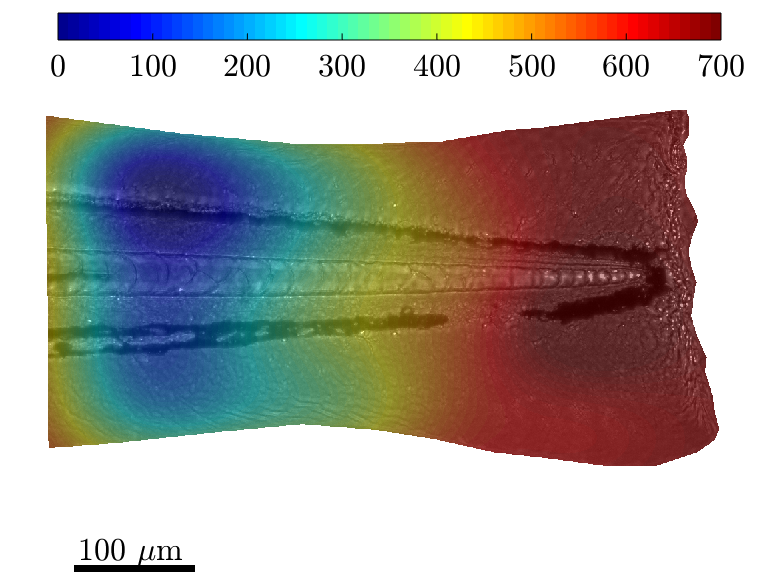
\includegraphics[width=.95\textwidth]{Figures/pruned_field_fish3.png}}\only<2>{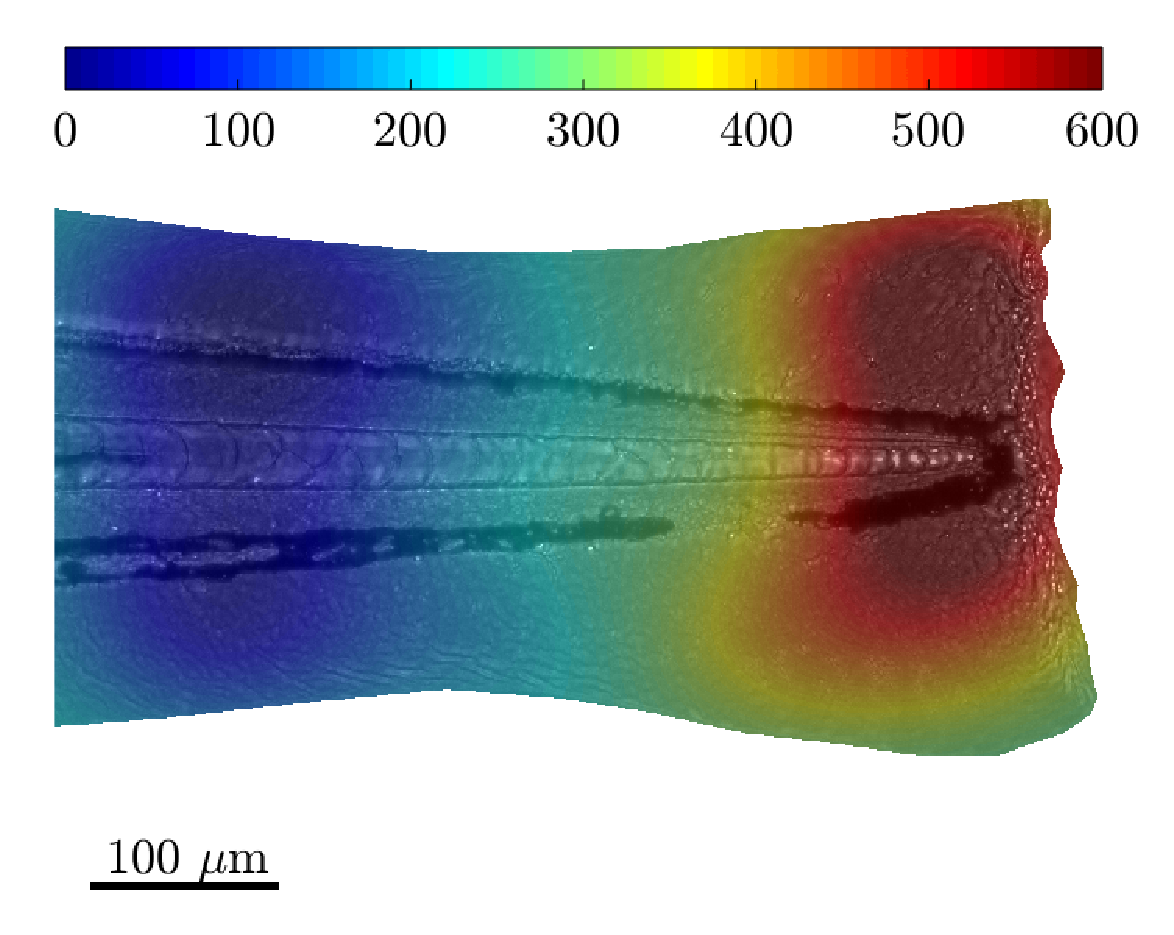
\includegraphics[width=.95\textwidth]{Figures/field_3.png}}};
	\node[block,align=center] at (10,3.25) (A8){\only<1>{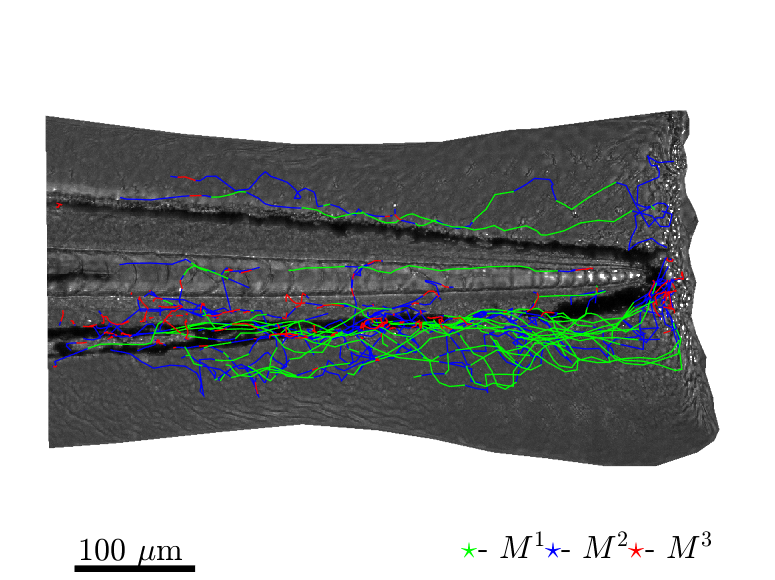
\includegraphics[width=.95\textwidth]{Figures/pruned_tracks_fish3.png}}\only<2>{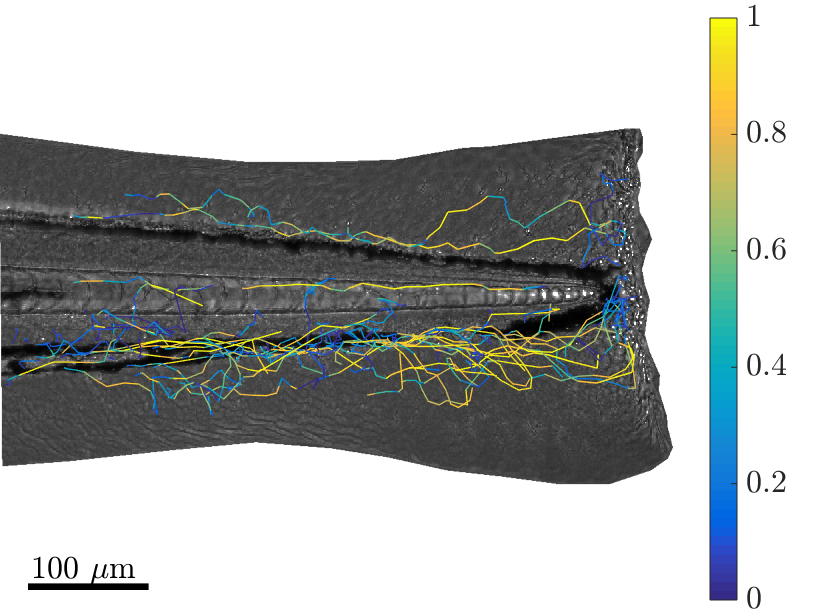
\includegraphics[width=.95\textwidth]{Figures/mode1_fish3.png}}};
	\draw[line width=0.5mm,cyan!70!black, rounded corners] (3.55,7.3) rectangle (7.95,1.8);
	\node at (3.7,6.2) (A9){};
	\node at (3.7,2.8) (A10){};
	\node at (3.7,4.45) (A11){};
	\node at (7.8,5.8) (A12){};
	\node at (7.8,3.25) (A13){};
	%% arrows
	\draw (A1) -- (A9); 
	\draw (A2) -- (A11); 
	\draw (A3) -- (A10); 
	\draw (A12) -- (A7); 
	\draw (A13) -- (A8); 
%	\path
%	(A5.east) edge[dashed,bend left=30] (A6.east);
	\path
	(A5.south) edge[dashed] (A15.north);
	\path
	(A15.south) edge[dashed] (A6.north);
	\path
	(A6.east) edge[dashed,bend right=30] (A5.east);
	\end{tikzpicture}
\end{figure}
\end{frame}

\subsection{Selected results}
\begin{frame}{Migratory modes - normal injury}
\begin{columns}
	\begin{column}{0.31\textwidth}
		\vspace{-0.2cm}
		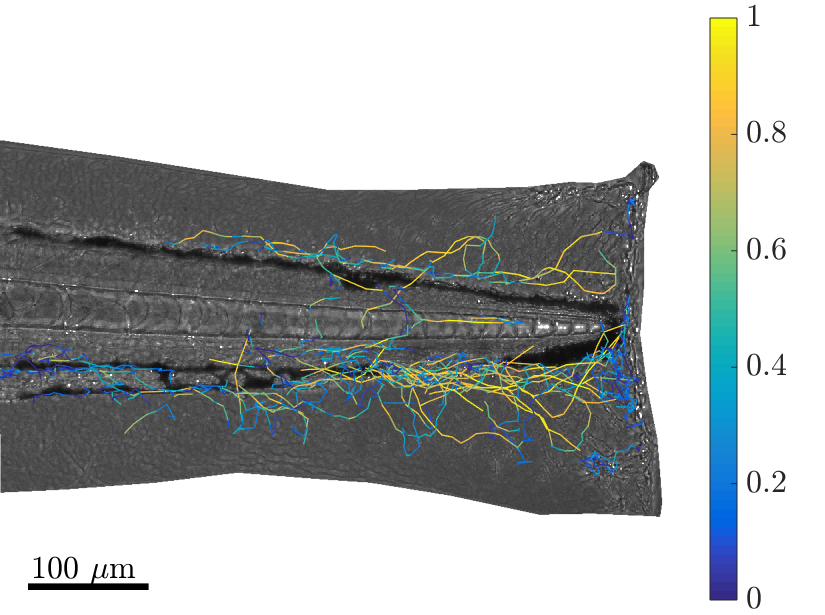
\includegraphics[scale=0.18]{Figures/mode1_fish1.png}\vfil
		\vspace{0.2cm}
		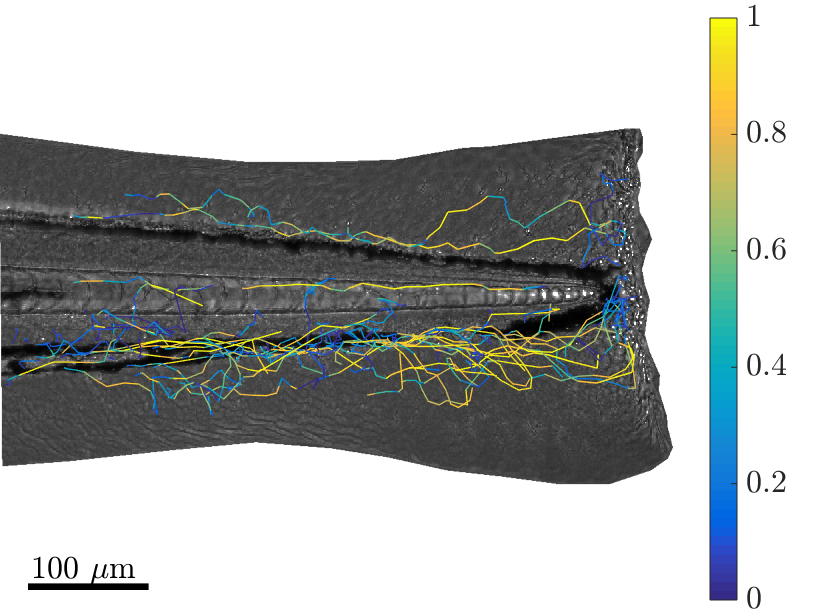
\includegraphics[scale=0.18]{Figures/mode1_fish3.png}
	\end{column}
	\begin{column}{0.31\textwidth}
		\vspace{-0.2cm}
		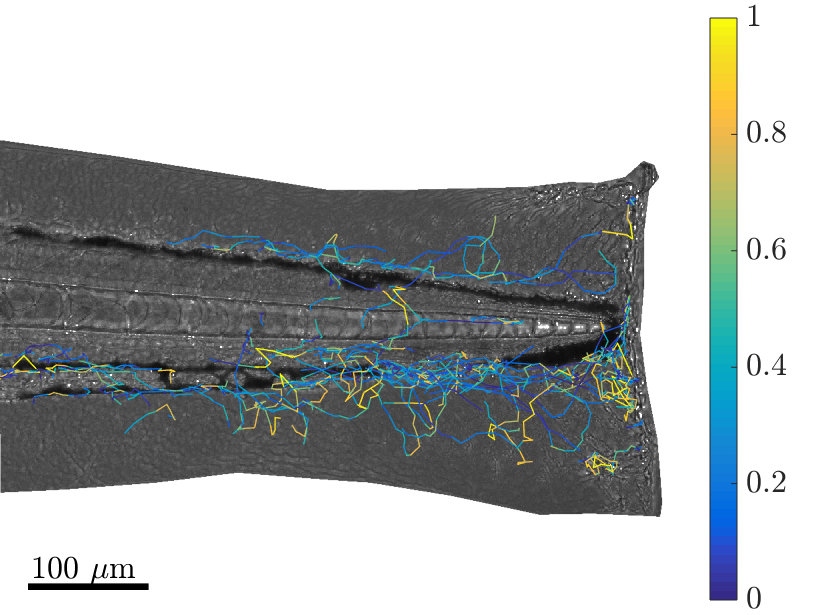
\includegraphics[scale=0.18]{Figures/mode2_fish1.png}\vfil
		\vspace{0.2cm}
		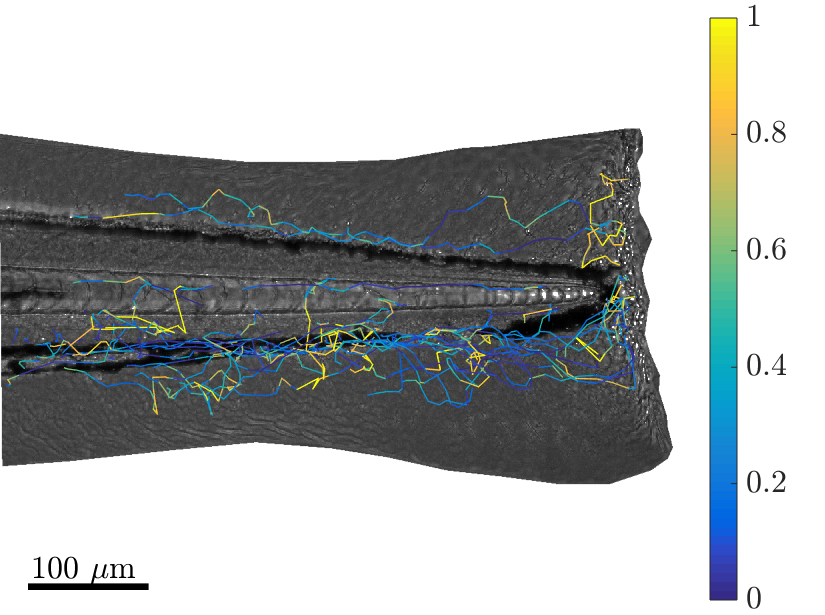
\includegraphics[scale=0.18]{Figures/mode2_fish3.png}
	\end{column}
	\begin{column}{0.31\textwidth}
		\vspace{-0.2cm}
		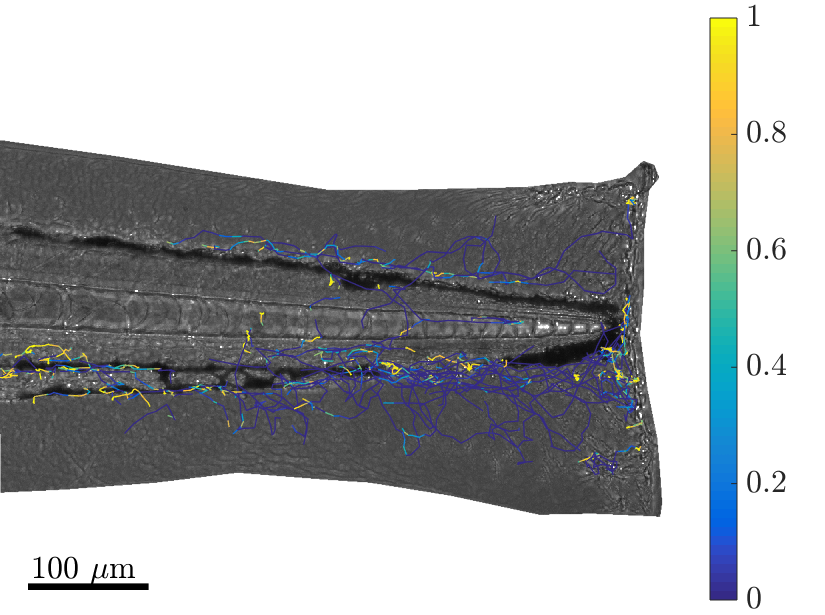
\includegraphics[scale=0.18]{Figures/mode3_fish1.png}\vfil
		\vspace{0.2cm}
		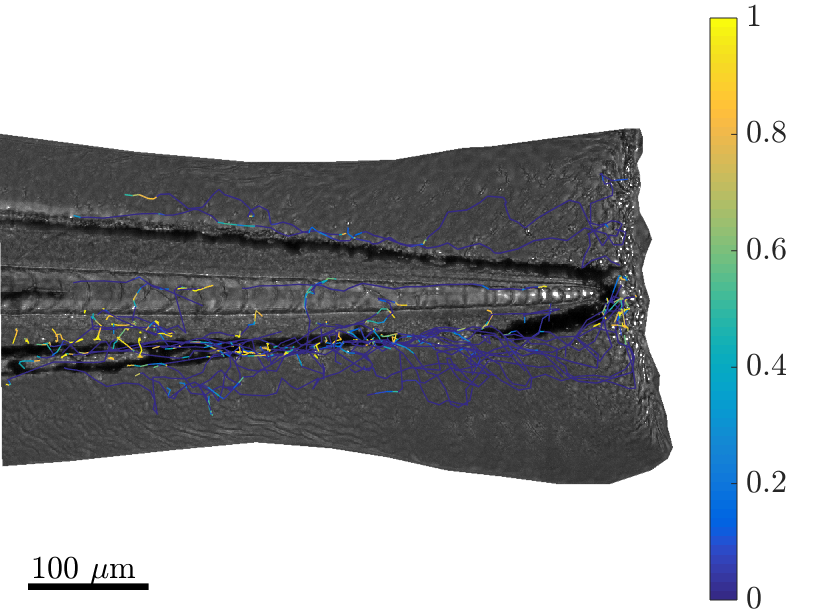
\includegraphics[scale=0.18]{Figures/mode3_fish3.png}
	\end{column}
\end{columns}
\begin{columns}
	\centering
	\begin{column}{0.31\textwidth}
		\centering
		\footnotesize{ a) $p(M^1)$}
	\end{column}
	\begin{column}{0.31\textwidth}
		\centering
		\footnotesize{ b)  $p(M^2)$}
	\end{column}
	\begin{column}{0.31\textwidth}
		\centering
		\footnotesize{ c)  $p(M^3)$}
	\end{column}
\end{columns}
\end{frame}
\begin{frame}{Estimated cell velocities}
\begin{columns}
	\begin{column}{0.32\textwidth}
		\scalebox{0.7}{\input{Tikzes/histogram_vx1_fish1.tikz}}\vfil
		\scalebox{0.7}{\input{Tikzes/histogram_vx1_fish3.tikz}}
	\end{column}
	\begin{column}{0.3\textwidth}
		\scalebox{0.7}{\input{Tikzes/histogram_vx2_fish1.tikz}}\vfil
		\scalebox{0.7}{\input{Tikzes/histogram_vx2_fish3.tikz}}
	\end{column}
	\begin{column}{0.3\textwidth}
		\scalebox{0.7}{\input{Tikzes/histogram_vx3_fish1.tikz}}\vfil
		\scalebox{0.7}{\input{Tikzes/histogram_vx3_fish3.tikz}}
	\end{column}
\end{columns}
\begin{columns}
	\centering
	\begin{column}{0.3\textwidth}
		\centering
		\footnotesize{ a) $M^1$}
	\end{column}
	\begin{column}{0.3\textwidth}
		\centering
		\footnotesize{ b) $M^2$}
	\end{column}
	\begin{column}{0.3\textwidth}
		\centering
		\footnotesize{ c) $M^3$}
	\end{column}
\end{columns}
\end{frame} 
%\begin{frame}{Migratory modes - severe and mild injury}
%\begin{columns}
%	\begin{column}{0.3\textwidth}
%		\vspace{-0.2cm}
%		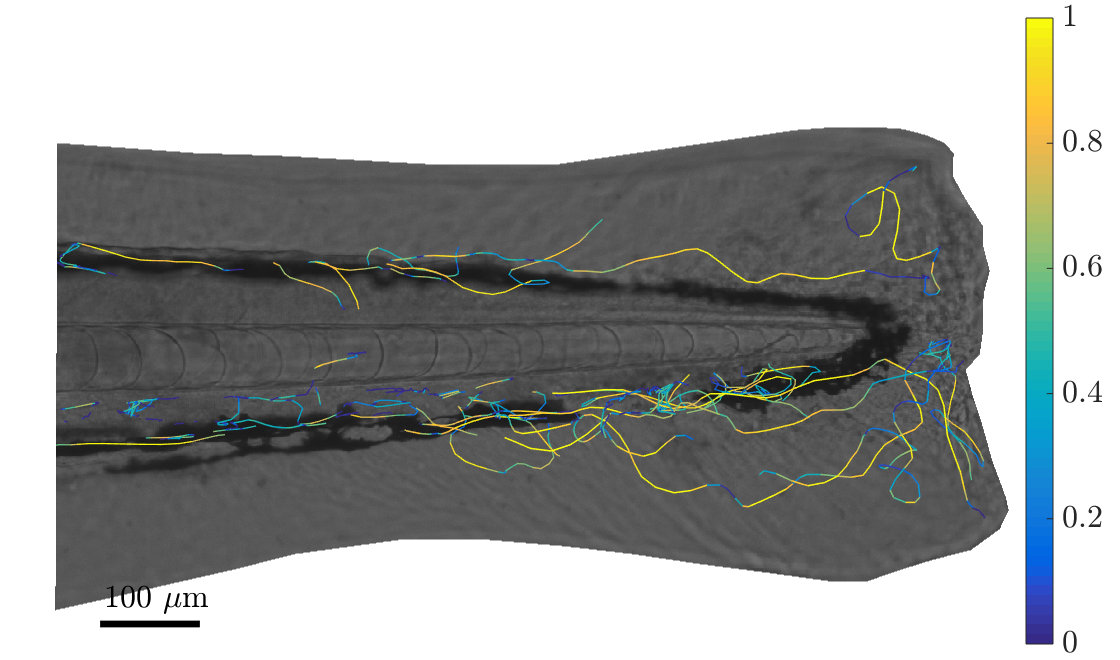
\includegraphics[scale=0.137]{Figures/mild1_mode1.png}\vfil
%		\vspace{0.2cm}
%		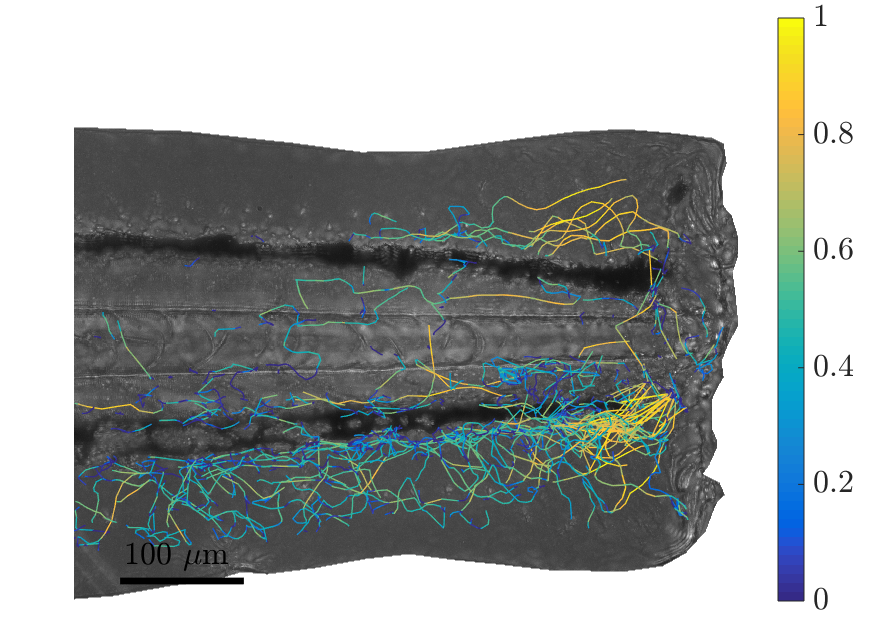
\includegraphics[scale=0.17]{Figures/severe1_mode1.png}
%	\end{column}
%	\begin{column}{0.3\textwidth}
%		\vspace{-0.2cm}
%		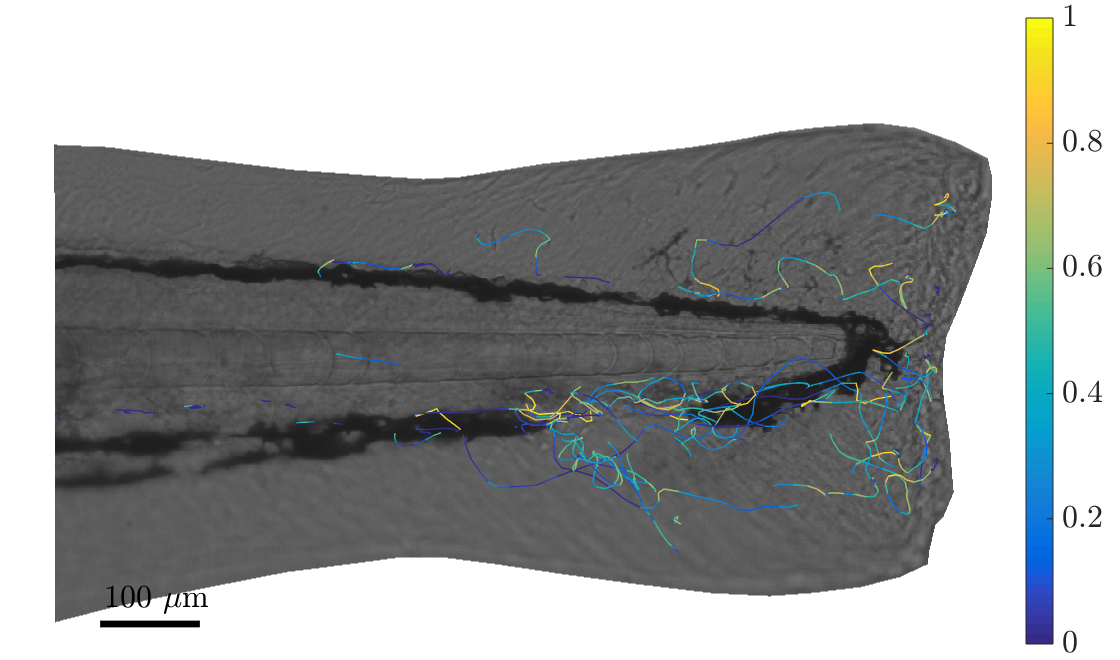
\includegraphics[scale=0.137]{Figures/mild1_mode2.png}\vfil
%		\vspace{0.2cm}
%		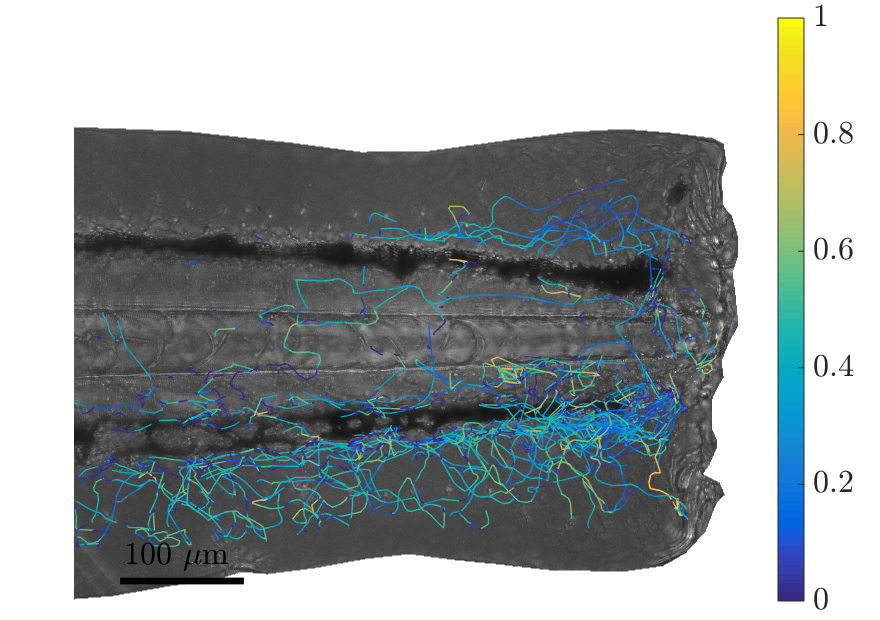
\includegraphics[scale=0.17]{Figures/severe1_mode2.png}
%	\end{column}
%	\begin{column}{0.3\textwidth}
%		\vspace{-0.2cm}
%		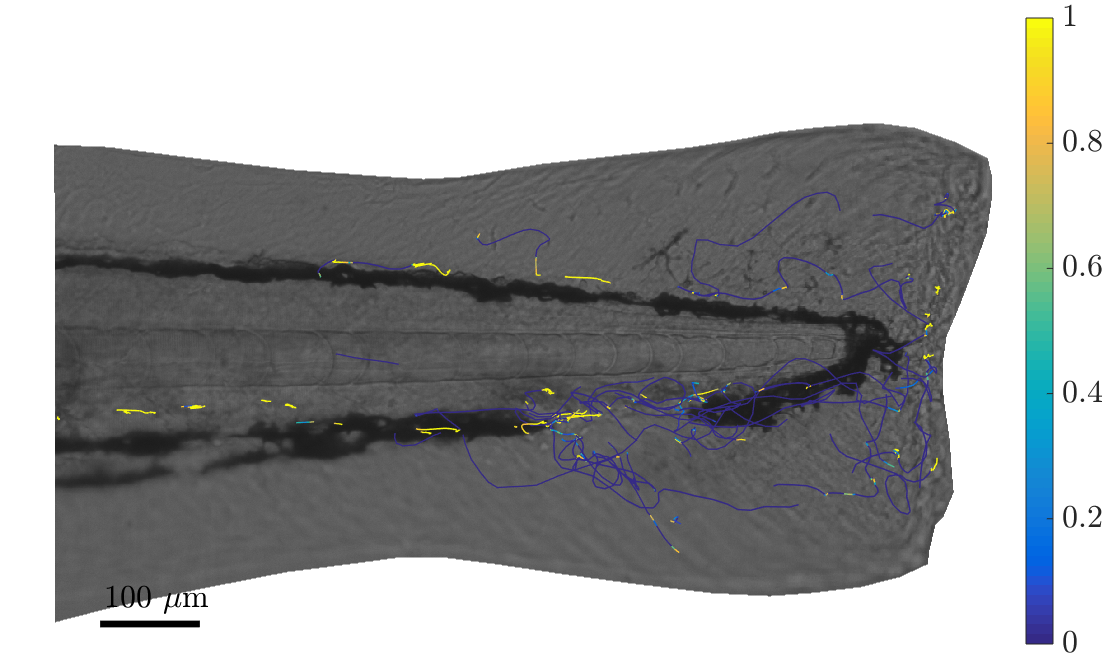
\includegraphics[scale=0.137]{Figures/mild1_mode3.png}\vfil
%		\vspace{0.2cm}
%		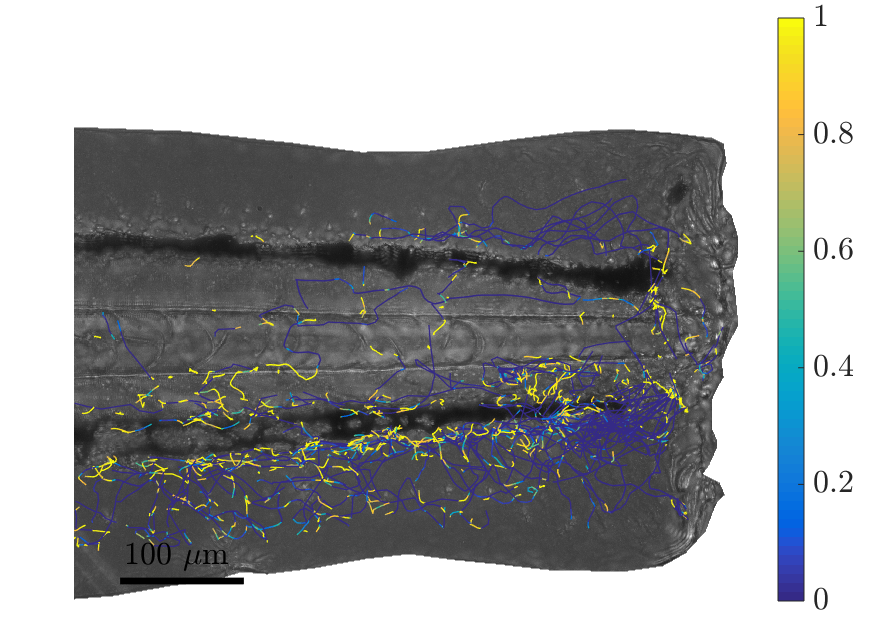
\includegraphics[scale=0.17]{Figures/severe1_mode3.png}
%	\end{column}
%\end{columns}
%\begin{columns}
%\centering
%\begin{column}{0.31\textwidth}
%	\centering
%	\footnotesize{ a) $p(M^1)$}
%\end{column}
%\begin{column}{0.3\textwidth}
%	\centering
%	\footnotesize{ b)  $p(M^2)$}
%\end{column}
%\begin{column}{0.3\textwidth}
%	\centering
%	\footnotesize{ c)  $p(M^3)$}
%\end{column}
%\end{columns}
%\end{frame}
%\begin{frame}{Inferred chemoattractant environment}
%\begin{columns}
%	\begin{column}{0.3\textwidth}
%		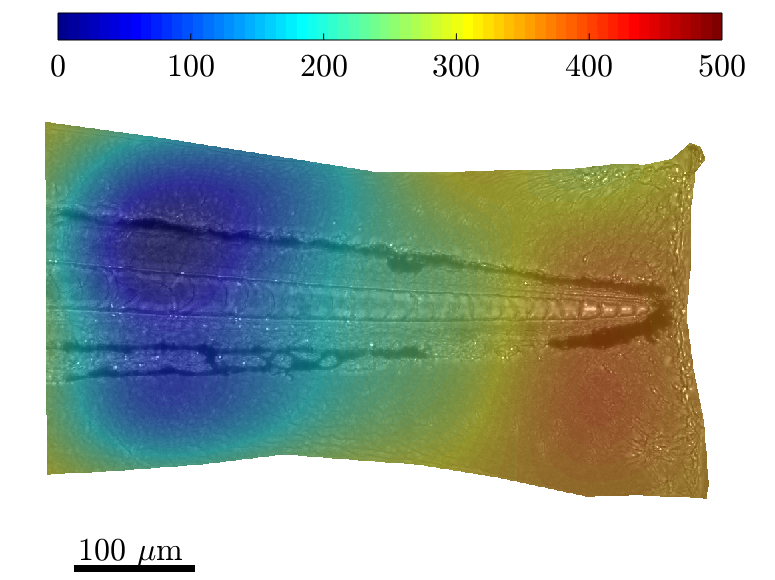
\includegraphics[scale=0.19]{Figures/field_fish1.png}
%		\vspace{0.4cm}
%		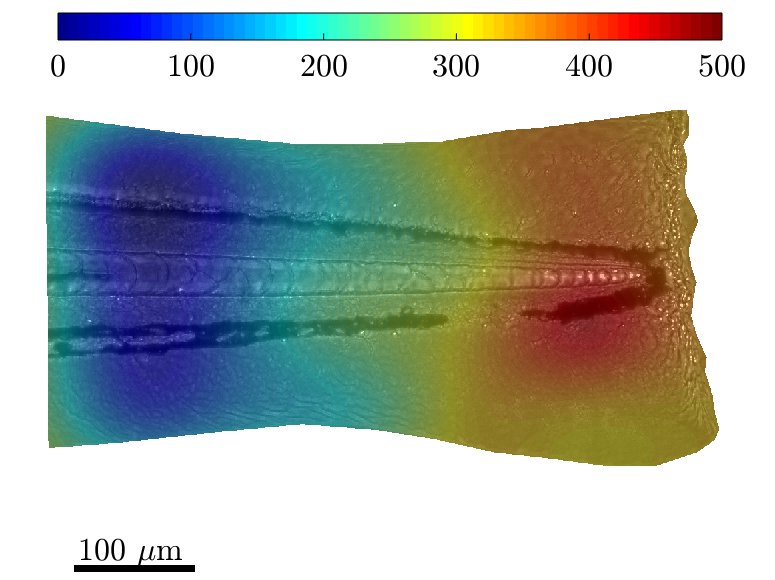
\includegraphics[scale=0.19]{Figures/field_fish3.png}
%	\end{column}
%	\begin{column}{0.3\textwidth}
%		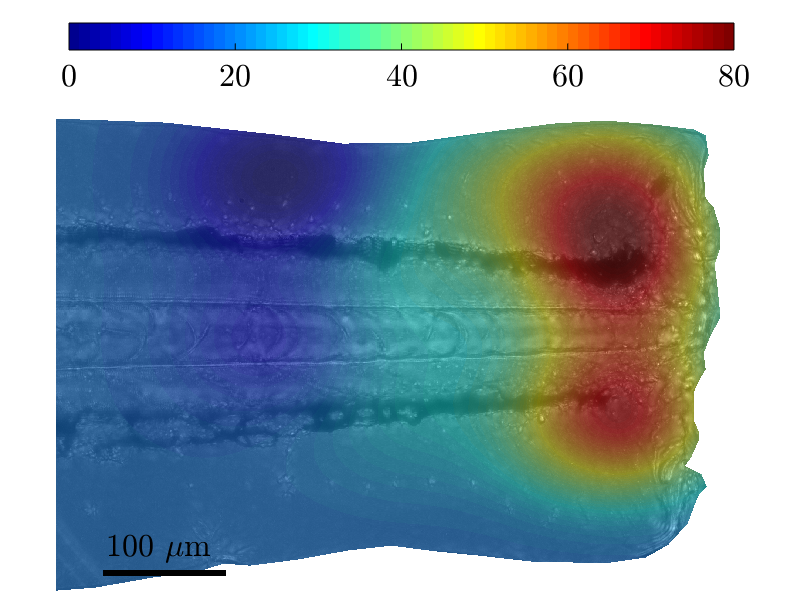
\includegraphics[scale=0.18]{Figures/severe1_field.png}
%		\vspace{0.3cm}
%		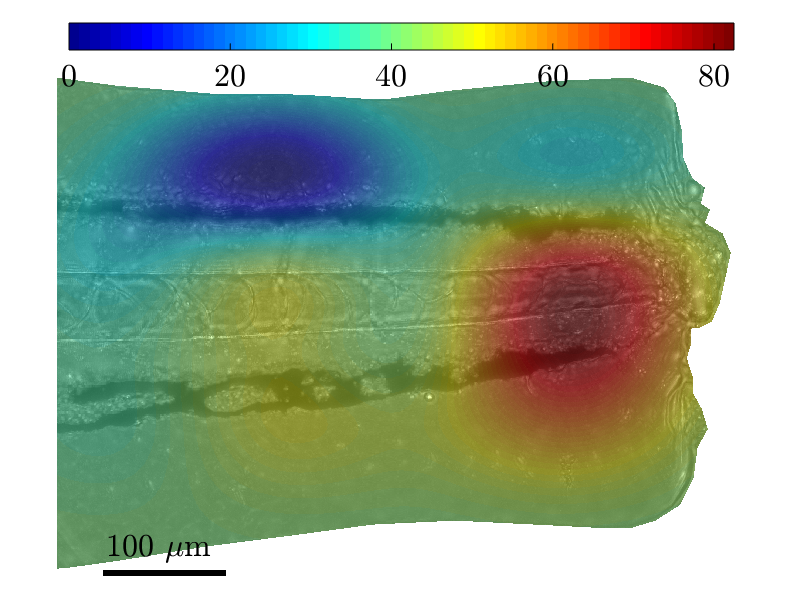
\includegraphics[scale=0.18]{Figures/severe2_field.png}
%	\end{column}
%	\begin{column}{0.3\textwidth}
%		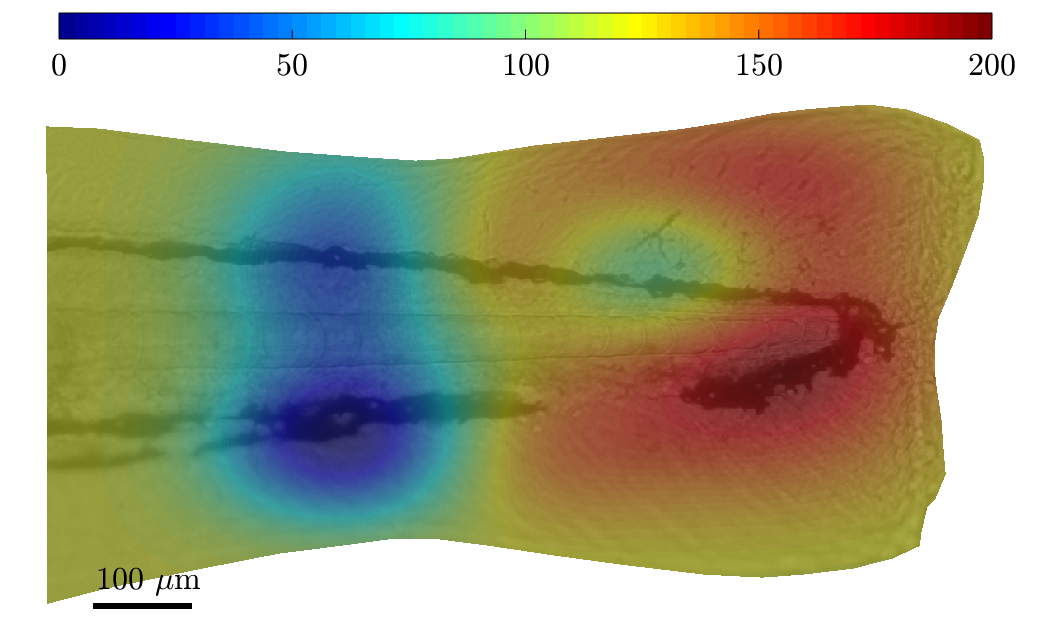
\includegraphics[scale=0.14]{Figures/mild1_field.png}
%		\vspace{0.6cm}
%		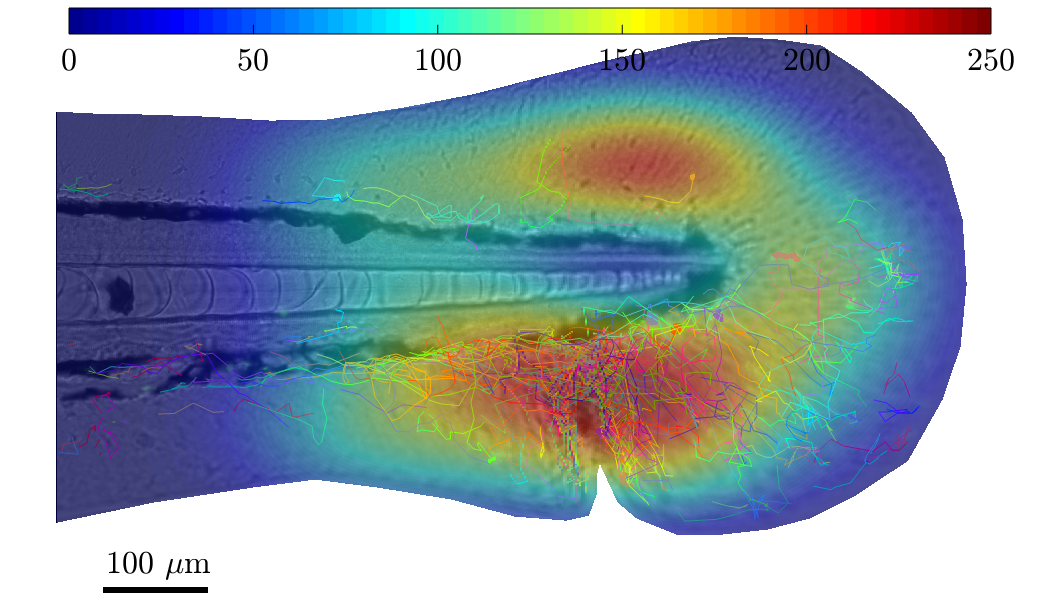
\includegraphics[scale=0.14]{Figures/nick4_field.png}
%	\end{column}
%\end{columns}
%\begin{columns}
%	\begin{column}{0.3\textwidth}
%		\centering
%		\footnotesize{ a) normal injury}
%	\end{column}
%	\begin{column}{0.3\textwidth}
%		\centering
%		\footnotesize{ b) severe injury}
%	\end{column}
%	\begin{column}{0.3\textwidth}
%		\centering
%		\footnotesize{ c) mild injury}
%	\end{column}
%\end{columns}
%\end{frame}
\begin{frame}{Reverse migration}
\begin{columns}
	\begin{column}{0.31\textwidth}
		\vspace{-0.2cm}
		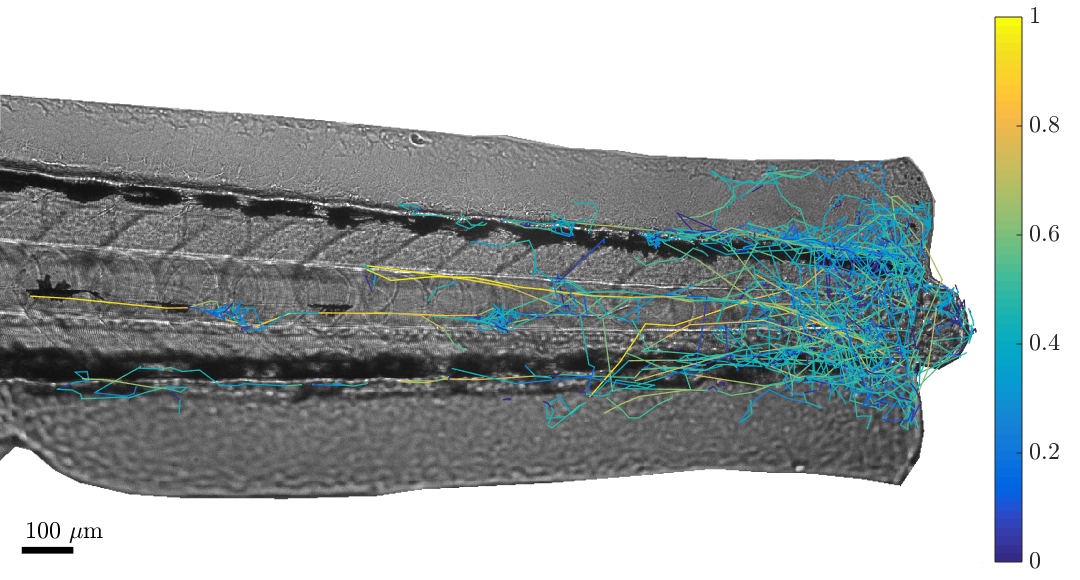
\includegraphics[scale=0.137]{Figures/mode1_rev2.png}\vfil
		\vspace{0.2cm}
		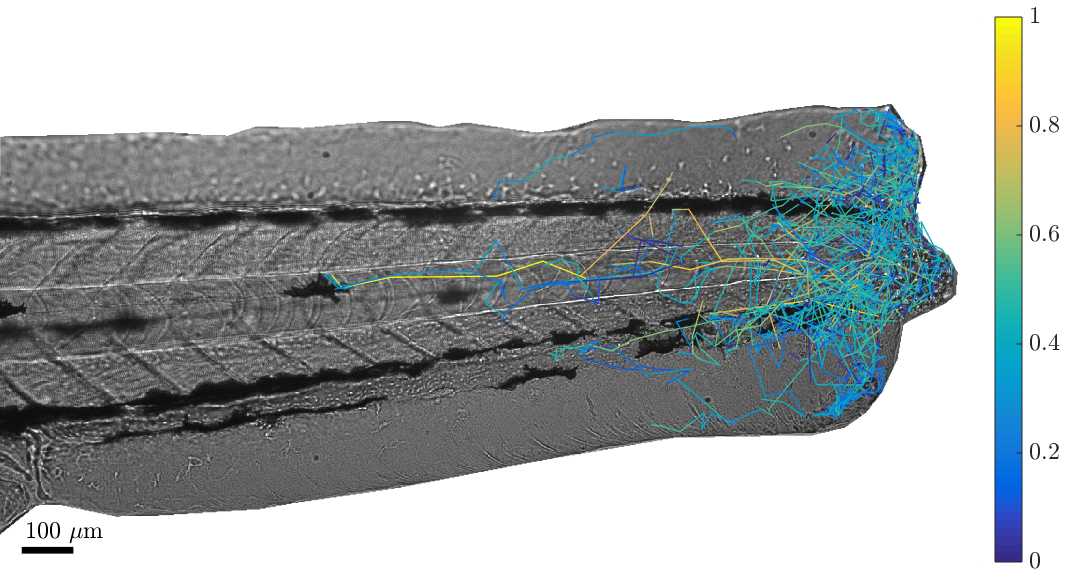
\includegraphics[scale=0.137]{Figures/mode1_rev9.png}
	\end{column}
	\begin{column}{0.31\textwidth}
		\vspace{-0.2cm}
		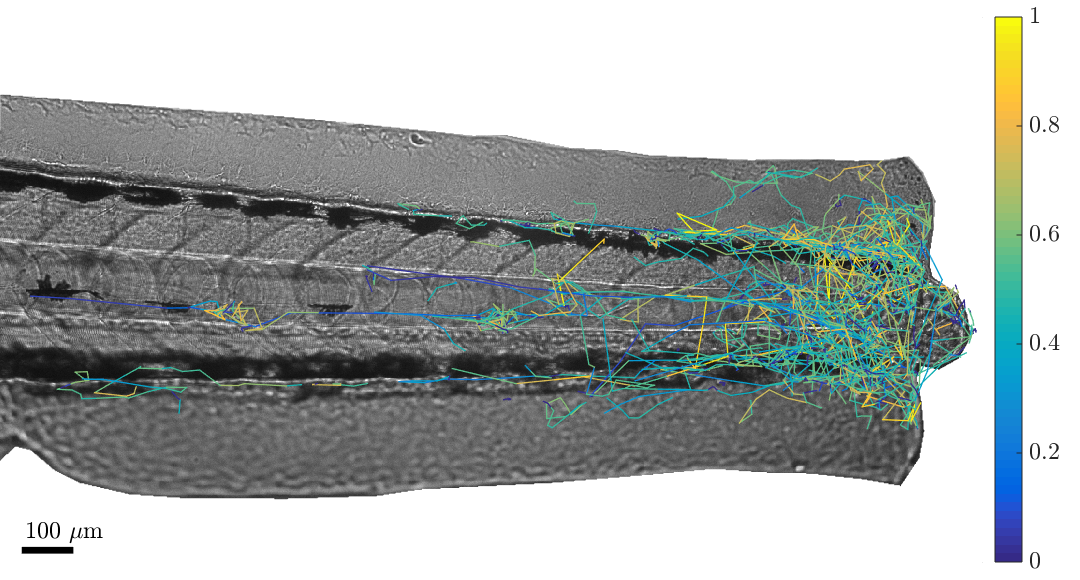
\includegraphics[scale=0.137]{Figures/mode2_rev2.png}\vfil
		\vspace{0.2cm}
		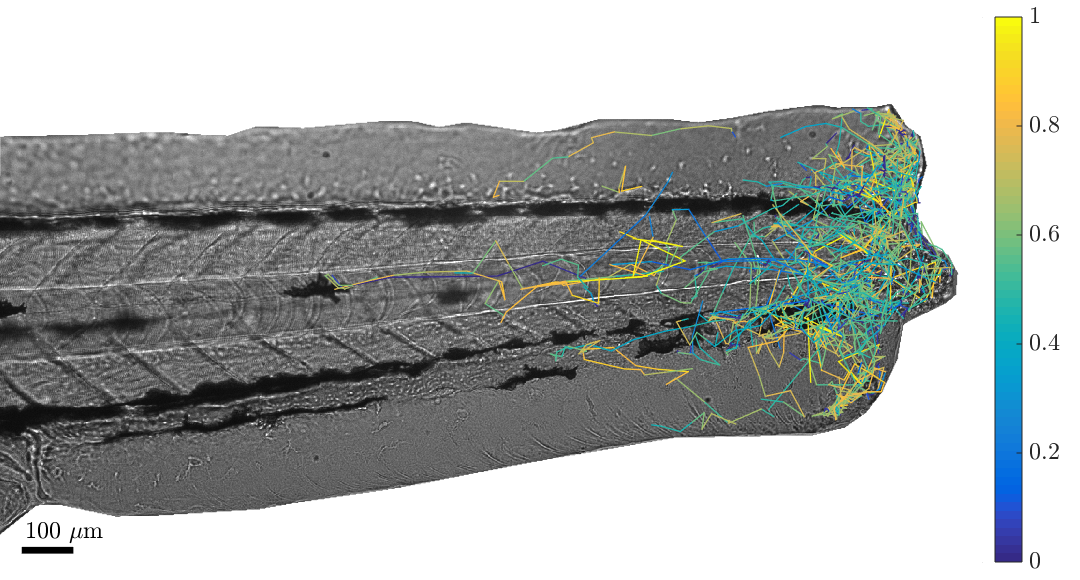
\includegraphics[scale=0.137]{Figures/mode2_rev9.png}
	\end{column}
	\begin{column}{0.31\textwidth}
		\vspace{-0.2cm}
		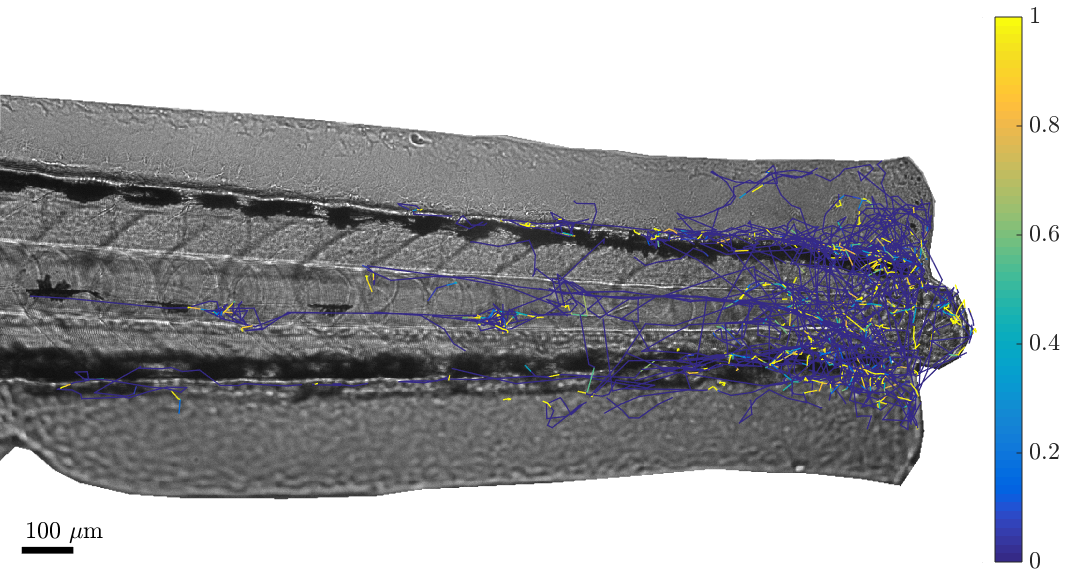
\includegraphics[scale=0.137]{Figures/mode3_rev2.png}\vfil
		\vspace{0.2cm}
		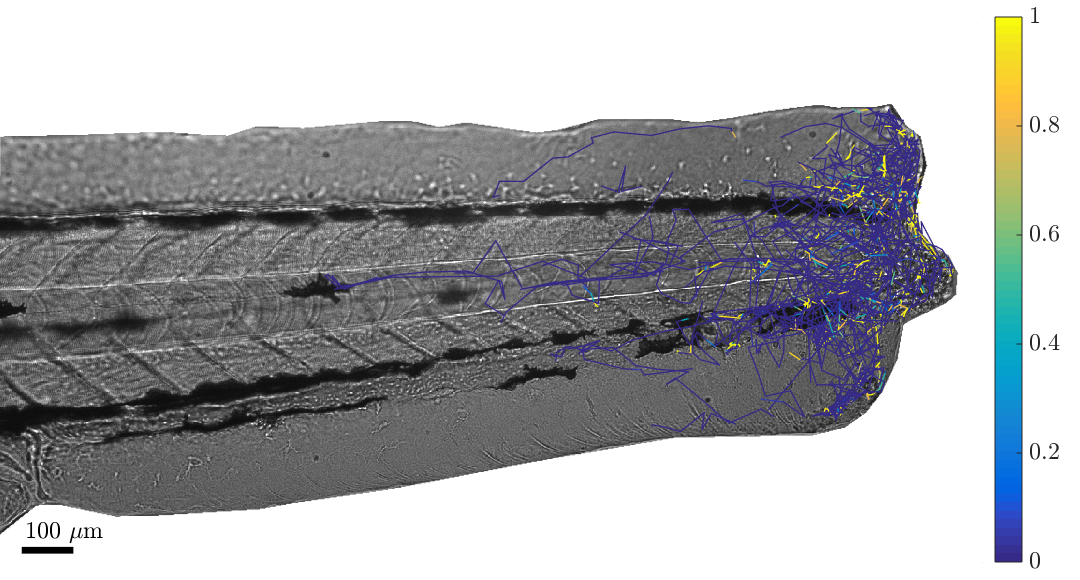
\includegraphics[scale=0.137]{Figures/mode3_rev9.png}
	\end{column}
\end{columns}
\begin{columns}
	\centering
	\begin{column}{0.31\textwidth}
		\centering
		\footnotesize{ a) $p(M^1)$}
	\end{column}
	\begin{column}{0.31\textwidth}
		\centering
		\footnotesize{ b)  $p(M^2)$}
	\end{column}
	\begin{column}{0.31\textwidth}
		\centering
		\footnotesize{ c)  $p(M^3)$}
	\end{column}
\end{columns}
\vspace{0.5cm}
For 4 datasets there is higher probability of neutrophils diffusing away from the wound.
\end{frame}

%%%%%%%%%%%%%%%%%%%%%%%%%%%%%%%%%%%%%%%%%%%%%%%%%%%%%%%%%%%%%%%%%%%%%%%%%%%%%%%%%%%%%%%%%%%%%%%%%%%%%%%%%%%%%%%%%%%
\section{Estimating cell morphodynamics}
\subsection{Problem statement}
\begin{frame}{Signal to migration}
\centering
\scalebox{1}{\input{Tikzes/RDS3.tikz}}
\vfil
\invisible<1-3>{Does PIP$_3$ activate pseudopod growth in migrating neutrophils?}
\invisible<1-4>{Does PIP$_3$ activate pseudopod growth in migrating neutrophils?}
\end{frame}
%\begin{frame}{Data}
%\vspace{-0.5cm}
%\centering
%\begin{tikzpicture}
%\node[text width=8em,text centered] at (0,0) {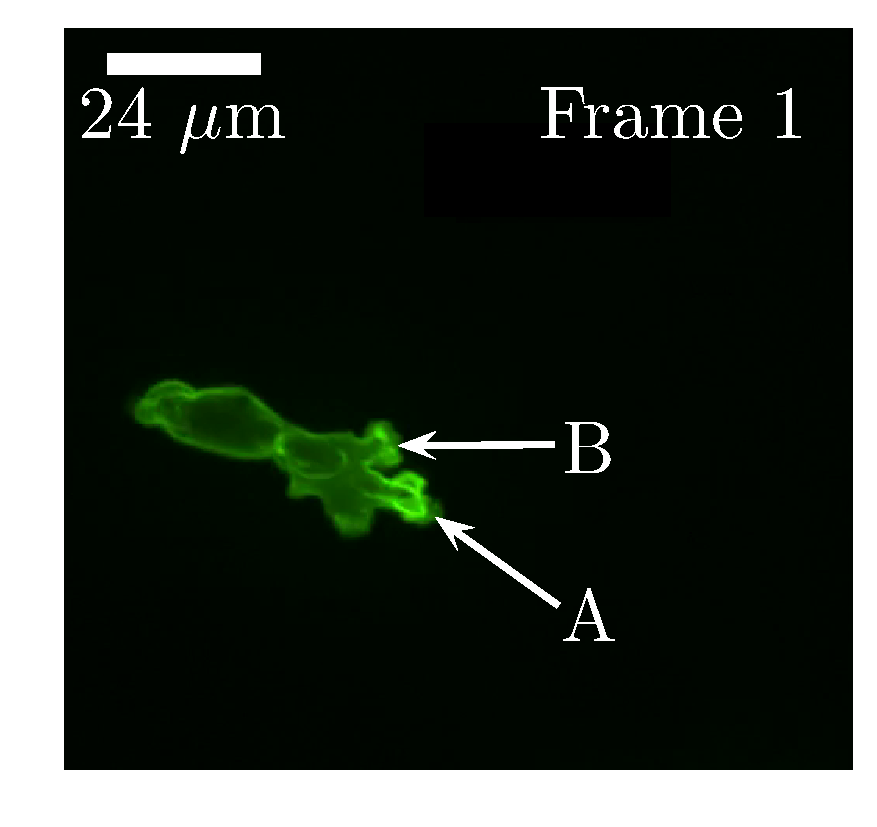
\includegraphics[width=\textwidth]{Figures/fr_1.eps}};
%\node[text width=8em,text centered] at (3,0) {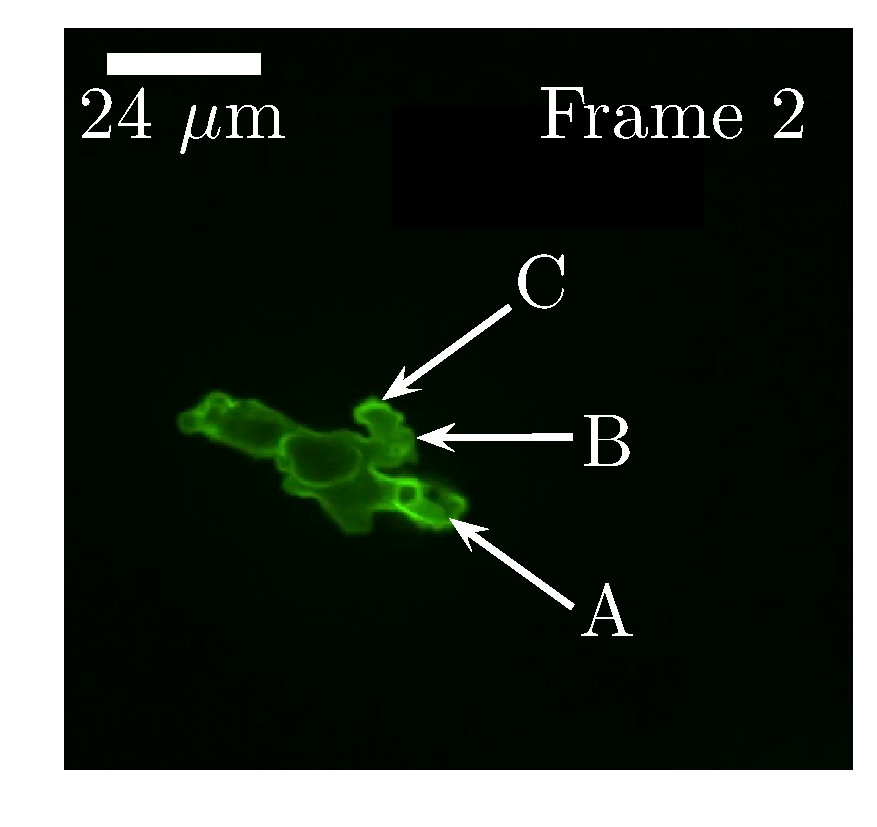
\includegraphics[width=\textwidth]{Figures/fr_2.eps}};
%\node[text width=8em,text centered] at (6,0) {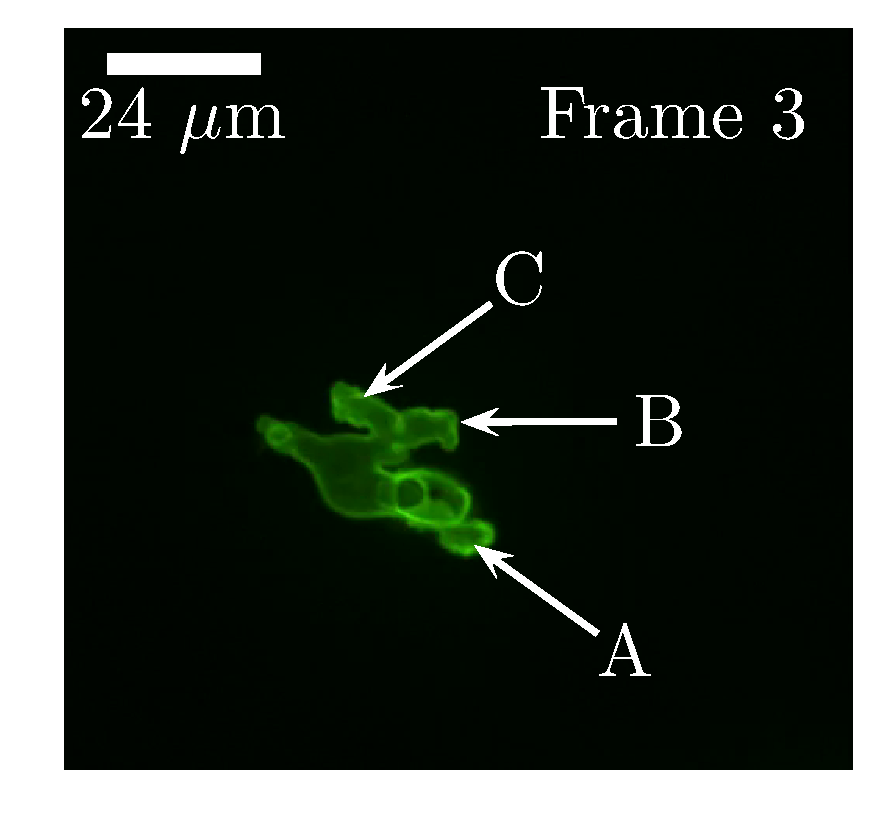
\includegraphics[width=\textwidth]{Figures/fr_3.eps}};
%\node[text width=8em,text centered] at (9,0) {\includegraphics[width=\textwidth]{Figures/fr_4.eps}};
%\node[text width=8em,text centered] at (0,-3) {\includegraphics[width=\textwidth]{Figures/fr_5.eps}};
%\node[text width=8em,text centered] at (3,-3) {\includegraphics[width=\textwidth]{Figures/fr_6.eps}};
%\node[text width=8em,text centered] at (6,-3) {\includegraphics[width=\textwidth]{Figures/fr_7.eps}};
%\node[text width=8em,text centered] at (9,-3) {\includegraphics[width=\textwidth]{Figures/fr_8.eps}};
%\end{tikzpicture}
%\end{frame}
\begin{frame}{Defining assumptions}
\begin{itemize}
	\item PIP$_3$ is the only activator regulating cell membrane protrusions.
	\item The integrated 
fluorescence intensity obtained from the imaging data is proportional to the local PIP$_3$ concentration.
	\item Local shape change is fully described by the evolution of local normal velocity.
	\begin{equation*}
	\mathbfit{v}_{\td+1}^{k} = \mathbfit{v}_{\td}^{k} + \frac{1}{m} \mathcal{F} + \mathbfit{w}_{\td}.
	\end{equation*}
	\item The cell is a 2-D curve $\Gamma_{\td}$. 3-D effects are accounted for in the random acceleration $\mathbfit{w}_{\td}$.
\end{itemize}
\end{frame}
\subsection{Methods}
\begin{frame}{Forces acting on cell boundary}
\begin{equation*}
\mathcal{F} = (\mathcal{F}_{\textrm{visc}} + \mathcal{F}_{\textrm{pro}} + \mathcal{F}_{\textrm{ten}} + \mathcal{F}_{\textrm{vol}})\nu,
\end{equation*}
\begin{itemize}
	\item \textbf{\textit{Protrusive force}} caused by acting regulators along the membrane: \begin{equation*}
	\mathcal{F}_{\textrm{pro}} = \alpha_{\textrm{pro}}\textrm{a}_{\td}^{k}.
	\end{equation*}
	\item \textbf{\textit{Surface tension}} prevents cell membrane from stretching:
	\begin{equation*}
	\mathcal{F}_{\textrm{ten}} = \alpha_{\textrm{ten}} \kappa_{\td}^{k}.
	\end{equation*} 
	\item \textbf{\textit{Volume conservation}} balances small volume changes:
	\begin{equation*}
	\mathcal{F}_{\textrm{vol}} = \alpha_{\textrm{vol}}\Delta\mathcal{A}_{\td}.
	\end{equation*} 
	\item \textbf{\textit{Viscous force}} opposes cell motion:
	\begin{equation*}
	\mathcal{F}_{\textrm{visc}} = -\alpha_{\textrm{vv}}v_{\td}^{k}.
	\end{equation*}
\end{itemize}
$\quad$\\
$\quad$
\end{frame}
%\begin{frame}{State space model}
%\vspace{-0.5cm}
%\begin{equation*}
%\Gamma_{\td}: \mathrm{s}_{\td}^{k}, \quad k = 1, \dots, K.
%\end{equation*}
%Local evolution for the node $\mathrm{s}_{\td}^{k}$:
%\begin{equation*}
%\mathbfit{v}_{\td+1}^{k} = A\mathbfit{v}_{\td}^{k} + B\mathbfit{u}_{\td}^{k}+ \mathbfit{w}_{\td}^{k}, \quad \mathbfit{w}{\td}^{k} \sim \mathcal{N}(0,Q).
%\end{equation*}
%\begin{equation*}
%\mathbfit{y}_{\td}^{k} = C \mathbfit{v}_{\td}^{k}.
%\end{equation*}
%\begin{itemize}
%\item 
%$A = 1 - \alpha_{\textrm{vv}}$;
%$B = \left[\alpha_{\textrm{pro}}, \alpha_{\textrm{ten}}, \alpha_{\textrm{vol}}\right]$;
%\item 
%$\mathbfit{u}_{\td}^{k} =\left[  a_{\td}^{k}, \kappa_{\td}^{k}, \Delta\mathcal{A}_{\td} \right] ^\top$, where
%	\begin{itemize}
%		\item $a_{\td}^{k}$ - local concentration of PIP$_3$;
%		\item $\kappa_{\td}^{k}$ - local curvature;
%		\item $\Delta\mathcal{A}_{\td} = \mathcal{A}_{\td} - \mathcal{A}_0$ - change in cell shape. 
%	\end{itemize}
%\item $\Theta = \lbrace A, B, Q, \mathbfit{v}_0, P_0 \rbrace$ - estimated via classic EM algorithm.
%\end{itemize}
%\end{frame}
\begin{frame}{Image processing framework}
\begin{figure}
	\centering
	\begin{tikzpicture}[->, >=stealth', auto, semithick, node distance=5em]
	\tikzstyle{block} = [rectangle, draw, fill=white, 
	text width=7em, text centered, rounded corners, minimum height=5.5em]
	\tikzstyle{line} = [draw, -latex']
%	\draw[>=triangle 45,draw=cyan!50!black,line width=1pt, <->] (4.8,6.5) -- (5.7,6.5);	
	\node[block,align=center] at (0,5.5) (A1){\includegraphics[width=0.8\textwidth]{Figures/cell3.png}};
	\node[block,align=center] at (3.5,5.5) (A2){\includegraphics[width=0.7\textwidth]{Figures/tracking_res.png}};
	\node[block,align=center] at (7,5.5) (A3){\includegraphics[width=0.7\textwidth]{Figures/pip3.png}};
	\node[block,align=center] at (0,3) (A4){\includegraphics[width=0.8\textwidth]{Figures/curv3.png}};
	\node[block,align=center] at (3.5,3) (A5){\includegraphics[width=0.8\textwidth]{Figures/area3.png}};
	\node[block,align=center] at (7,3) (A6){\includegraphics[width=0.8\textwidth]{Figures/normvel3.png}};
	\node[block,align=center] at (0,0.5) (A7){\tiny $\mathbfit{x}_{\td+1}^{k} = A\mathbfit{x}_{\td}^{k} + B\mathbfit{u}_{\td}^{k}+ \mathbfit{w}_{\td}^{k};$\\ \tiny $\mathbfit{x}_{\td}^{k} = v_{\td}^{k}, k=1,\dots,K$;\\
	\tiny $\mathbfit{u}_{\td}^{k} =\left[  \textrm{a}_{\td}^{k}, \kappa_{\td}^{k}, \Delta\mathcal{A}_{\td} \right] ^\top.$};
	\node[block,align=center] at (3.5,0.5) (A8){\scriptsize $\Theta = \lbrace A, B, Q, \mathbfit{x}_0, P_0 \rbrace$};
	\node[block,align=center] at (7,0.5) (A9){\scriptsize $\mathcal{Q}^i = \E\left[ \log p(\mathcal{X} \mid \hat{\Theta}^{i})\right]; $\\ \scriptsize $\hat{\Theta}^{i+1} = \arg \underset{\Theta}{\max}\mathcal{Q}^i.$};
	\node at (9.2,5.5) (N1){};
	\node at (-2.2,3) (N2){};
	\node at (9.2,3) (N3){};
	\node at (-2.2,0.5) (N4){};
	\path
	(A1.east) edge[] (A2.west) 
	(A2.east) edge[] node[midway, above] {$v^{k}_{\nu,\td}$} (A3.west) 
	(A3.east) edge[] node[midway, above] {$\textrm{a}^{k}_{\td}$} (N1) 
	(N2) edge[] (A4.west)
	(A4.east) edge[] node[midway, above] {$\kappa^{k}_{\td}$} (A5.west)
	(A5.east) edge[] node[midway, above] {$\mathcal{A}_{\td}$} (A6.west)
	(A6.east) edge[] node[midway, above] {$v^{k}_{\nu,\td}$} (N3) 
	(N4) edge[] (A7.west)
	(A7.east) edge[] (A8.west)
	(A8.east) edge[] (A9.west);
	\end{tikzpicture}
\end{figure}
\end{frame}
%\begin{frame}{Image processing}
%\centering
%\includegraphics[scale=0.2]{Figures/motile_cell_t10.png}
%\vfil
%\includegraphics[scale=0.2]{Figures/motile_cell_t11.png}
%\end{frame}

\subsection{Selected results}
\begin{frame}{Motile cells observed in vivo}
\begin{columns}
	\begin{column}{0.48\textwidth}
		\centering
		\scalebox{0.6}{\input{Tikzes/histogram7.tikz}}	
	\end{column}
	\begin{column}{0.5\textwidth}
		\centering
		\begin{itemize}
			\item Very weak correlation between between $a_{\td-1}^{k}$ and $v_{\td}^{k}$ for all cells;
			\item Mann-Whitney test results: higher concentrations of PIP$_3$ correspond to accelerated protrusion growth.
			\item Results in agreement with recent knock-out studies.
		\end{itemize}
	\end{column}
\end{columns}
\end{frame}
%\begin{frame}{Motile cells observed in vivo}
%\begin{columns}
%	\begin{column}{0.35\textwidth}
%		\centering
%		\includegraphics[scale=0.3]{Figures/m4_akt.png}\vfil
%		\footnotesize{a) Smoothed intensity.}
%		\vfil
%		\includegraphics[scale=0.3]{Figures/m4_curvature.png}\vfil	
%		\footnotesize{a) Local curvature.}
%	\end{column}
%	\begin{column}{0.35\textwidth}
%		\centering
%		\includegraphics[scale=0.3]{Figures/m4_estimated_velocity.png}\vfil
%		\footnotesize{c) Estimated velocity.}
%		\vfil
%		\includegraphics[scale=0.3]{Figures/m4_modelled_velocity.png}\vfil
%		\footnotesize{d) Predicted velocity.}
%	\end{column}
%\end{columns}
%\end{frame}
\begin{frame}{Polarised cell observed in vitro}
\centering
\includegraphics[scale=0.385]{Figures/in_vitro_cell.png}
\vfil
\includegraphics[scale=0.195]{Figures/normally_polarised_t9.png}
\end{frame}
\begin{frame}{Polarised cell observed in vitro}
\begin{columns}
	\begin{column}{0.35\textwidth}
	\centering
	\includegraphics[scale=0.3]{Figures/polarised_smoothed_akt.png}\vfil
	\footnotesize{a) Smoothed intensity.}
	\vfil
	\includegraphics[scale=0.3]{Figures/polarised_curvature.png}\vfil	
	\footnotesize{a) Local curvature.}
\end{column}
\begin{column}{0.35\textwidth}
	\centering
	\includegraphics[scale=0.3]{Figures/polarised_estimated_velocity.png}\vfil
	\footnotesize{c) Estimated velocity.}
	\vfil
	\includegraphics[scale=0.3]{Figures/polarised_modelled_velocity.png}\vfil
	\footnotesize{d) Predicted velocity.}
\end{column}
\end{columns}
\end{frame}



\section{Conclusion}
\subsection{Contributions}
\begin{frame}{Technical contributions}
\begin{itemize}
	\item A reconfigurable hybrid model of individual cell dynamics that incorporates the influence of the global  environment.
	\item A statistical framework for simultaneous inference of the global chemoattractant environment and cell behavioural modes.
	\item An image processing and estimation framework that links local cell boundary evolution to observed subcellular concentrations.
\end{itemize}
\end{frame}
\begin{frame}{Contributions in field of application}
\begin{itemize}
	\item Investigation of neutrophil-environment interaction on different stages of inflammation.
	\item Quantitative evidence that the dominant mode of neutrophil reverse migration is random walk.
	\item Quantitative evidence that PIP$_3$ does not activate protrusions but accelerates existing leading edges in cells performing chemotaxis.
\end{itemize}
\end{frame}
\subsection{Future work}
\begin{frame}{Future work}
\begin{itemize}
	\item Utilising hierarchical/multi-resolution basis functions in environment decomposition.
	\item Introducing priors for the field parameters and Bayesian inference.
	\item Considering time-varying environment for recruitment stage of inflammation.
	\item Considering competing gradients for resolution stage of inflammation.
\end{itemize}
\end{frame}
\begin{frame}{Disseminated results}
\footnotesize{
\begin{itemize}
\item A. Kadochnikova, H.M. Isles, S.A. Renshaw, V. Kadirkamanathan.
"Estimation of Hidden Chemoattractant Field from Observed Cell Migration Patterns". A peer-reviewed paper in \textit{Proceedings of 18th IFAC Symposium on System Identification SYSID 2018}.
\item H.M. Isles, C. Muir, A. Kadochnikova, C.A. Loynes, V. Kadirkamanathan, P.M. Elks, S.A. Renshaw. "Non-apoptotic pioneer neutrophils initiate a swarming response in a zebrafish tissue injury model" under review in eLife Reports, 2019.
\end{itemize} 
In preparation:
\begin{itemize}
	\item A. Kadochnikova, V. Kadirkamanathan.
	"An Approximate Maximum Likelihood Framework for Estimating the Environment Driving multiple objects with Hybrid Dynamics".
	\item A. Kadochnikova, H.M. Isles, S.A. Renshaw, V. Kadirkamanathan. "Inference of the
	External Stimuli Environments from Heterogeneous Behaviour of Migrating Neutrophils in Zebrafish Model of Inflammation".
\end{itemize}
}
\end{frame}
\begin{frame}
\centering
\Huge{Thank you!}\\
\huge{Questions?}
\end{frame}
% All of the following is optional and typically not needed. 
%\appendix
%\section<presentation>*{\appendixname}
%\subsection<presentation>*{References}
%
%\begin{frame}[allowframebreaks]
%\printbibliography
%\end{frame}
\end{document}


